\documentclass{article}\usepackage[]{graphicx}\usepackage[]{color}
%% maxwidth is the original width if it is less than linewidth
%% otherwise use linewidth (to make sure the graphics do not exceed the margin)
\makeatletter
\def\maxwidth{ %
  \ifdim\Gin@nat@width>\linewidth
    \linewidth
  \else
    \Gin@nat@width
  \fi
}
\makeatother

\definecolor{fgcolor}{rgb}{0.345, 0.345, 0.345}
\newcommand{\hlnum}[1]{\textcolor[rgb]{0.686,0.059,0.569}{#1}}%
\newcommand{\hlstr}[1]{\textcolor[rgb]{0.192,0.494,0.8}{#1}}%
\newcommand{\hlcom}[1]{\textcolor[rgb]{0.678,0.584,0.686}{\textit{#1}}}%
\newcommand{\hlopt}[1]{\textcolor[rgb]{0,0,0}{#1}}%
\newcommand{\hlstd}[1]{\textcolor[rgb]{0.345,0.345,0.345}{#1}}%
\newcommand{\hlkwa}[1]{\textcolor[rgb]{0.161,0.373,0.58}{\textbf{#1}}}%
\newcommand{\hlkwb}[1]{\textcolor[rgb]{0.69,0.353,0.396}{#1}}%
\newcommand{\hlkwc}[1]{\textcolor[rgb]{0.333,0.667,0.333}{#1}}%
\newcommand{\hlkwd}[1]{\textcolor[rgb]{0.737,0.353,0.396}{\textbf{#1}}}%

\usepackage{framed}
\makeatletter
\newenvironment{kframe}{%
 \def\at@end@of@kframe{}%
 \ifinner\ifhmode%
  \def\at@end@of@kframe{\end{minipage}}%
  \begin{minipage}{\columnwidth}%
 \fi\fi%
 \def\FrameCommand##1{\hskip\@totalleftmargin \hskip-\fboxsep
 \colorbox{shadecolor}{##1}\hskip-\fboxsep
     % There is no \\@totalrightmargin, so:
     \hskip-\linewidth \hskip-\@totalleftmargin \hskip\columnwidth}%
 \MakeFramed {\advance\hsize-\width
   \@totalleftmargin\z@ \linewidth\hsize
   \@setminipage}}%
 {\par\unskip\endMakeFramed%
 \at@end@of@kframe}
\makeatother

\definecolor{shadecolor}{rgb}{.97, .97, .97}
\definecolor{messagecolor}{rgb}{0, 0, 0}
\definecolor{warningcolor}{rgb}{1, 0, 1}
\definecolor{errorcolor}{rgb}{1, 0, 0}
\newenvironment{knitrout}{}{} % an empty environment to be redefined in TeX

\usepackage{alltt}
% !Rnw weave = knitr
\usepackage[top=0.7in, bottom=0.7in, left=0.7in, right=0.5in]{geometry}
\usepackage[parfill]{parskip}
\IfFileExists{upquote.sty}{\usepackage{upquote}}{}

\begin{document}

% Need to have cash=false here




\title{Principles of Modelling and Simulation in Epidemiology}
% \subtitle{Laboratory exercise 2}
\author{Andreas Karlsson}
\maketitle


\bf{Required R-packages}
\begin{knitrout}
\definecolor{shadecolor}{rgb}{0.969, 0.969, 0.969}\color{fgcolor}\begin{kframe}
\begin{alltt}
\hlkwd{require}\hlstd{(deSolve)}  \hlcom{#For the deterministic solutions (also for initial and environmental stochasticity)}
\hlkwd{require}\hlstd{(GillespieSSA)}  \hlcom{#Gillespie Stochastic Simulation Algorithm with 'Explicit tau-leap'}
\hlcom{## More info at http://www.jstatsoft.org/v25/i12/paper}
\hlkwd{require}\hlstd{(ggplot2)}  \hlcom{#Extravagant plotting tool (not necessary to answer the questions)}
\hlkwd{require}\hlstd{(plyr)}  \hlcom{#Handy data manipulation tool (not necessary to answer the questions)}
\end{alltt}
\end{kframe}
\end{knitrout}


\bf{2.1 RNGs}
\begin{knitrout}
\definecolor{shadecolor}{rgb}{0.969, 0.969, 0.969}\color{fgcolor}\begin{kframe}
\begin{alltt}
\hlcom{## Uniform}
\hlkwd{layout}\hlstd{(}\hlkwd{matrix}\hlstd{(}\hlkwd{c}\hlstd{(}\hlnum{1}\hlstd{,} \hlnum{2}\hlstd{),} \hlnum{1}\hlstd{,} \hlnum{2}\hlstd{,} \hlkwc{byrow} \hlstd{=} \hlnum{TRUE}\hlstd{))}
\hlstd{unif} \hlkwb{<-} \hlkwd{runif}\hlstd{(}\hlkwc{n} \hlstd{=} \hlnum{10000}\hlstd{,} \hlkwc{min} \hlstd{=} \hlnum{5}\hlstd{,} \hlkwc{max} \hlstd{=} \hlnum{15}\hlstd{)}
\hlkwd{plot}\hlstd{(unif,} \hlkwc{ylim} \hlstd{=} \hlkwd{c}\hlstd{(}\hlnum{0}\hlstd{,} \hlnum{20}\hlstd{),} \hlkwc{pch} \hlstd{=} \hlstr{"."}\hlstd{)} \hlopt{+} \hlkwd{abline}\hlstd{(}\hlkwc{h} \hlstd{=} \hlkwd{mean}\hlstd{(unif),} \hlkwc{col} \hlstd{=} \hlnum{2}\hlstd{,} \hlkwc{lwd} \hlstd{=} \hlnum{3}\hlstd{)}
\hlkwd{hist}\hlstd{(unif)}
\end{alltt}
\end{kframe}
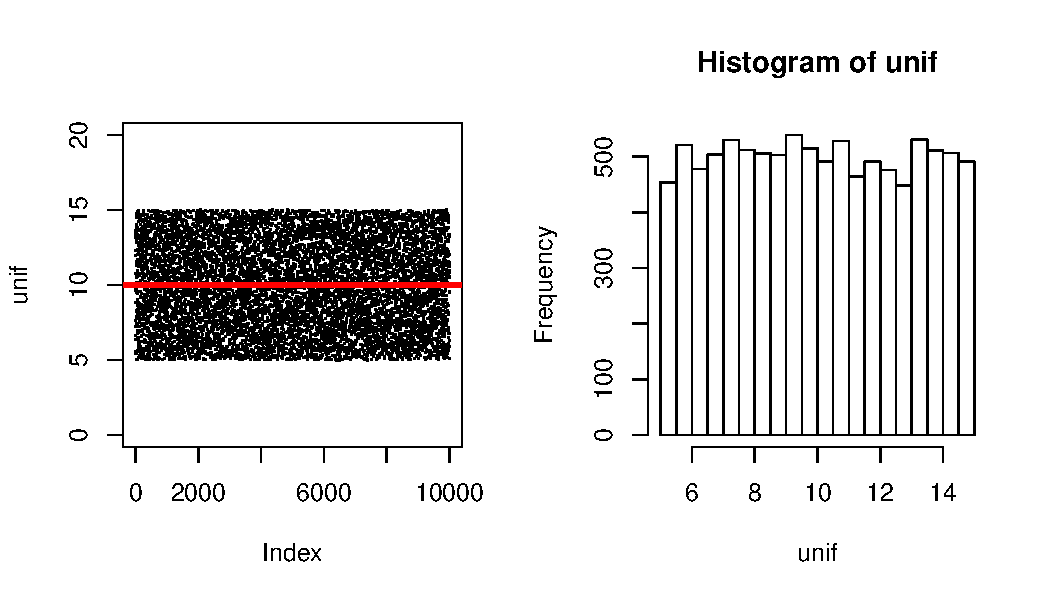
\includegraphics[width=.5\linewidth]{figure/RNG1} 
\begin{kframe}\begin{alltt}
\hlcom{## Exponential}
\hlstd{expo} \hlkwb{<-} \hlkwd{rexp}\hlstd{(}\hlkwc{n} \hlstd{=} \hlnum{10000}\hlstd{,} \hlkwc{rate} \hlstd{=} \hlnum{4}\hlstd{)}
\hlkwd{plot}\hlstd{(expo,} \hlkwc{pch} \hlstd{=} \hlstr{"."}\hlstd{)} \hlopt{+} \hlkwd{abline}\hlstd{(}\hlkwc{h} \hlstd{=} \hlkwd{mean}\hlstd{(expo),} \hlkwc{col} \hlstd{=} \hlnum{2}\hlstd{,} \hlkwc{lwd} \hlstd{=} \hlnum{3}\hlstd{)}
\hlkwd{hist}\hlstd{(expo)}
\end{alltt}
\end{kframe}
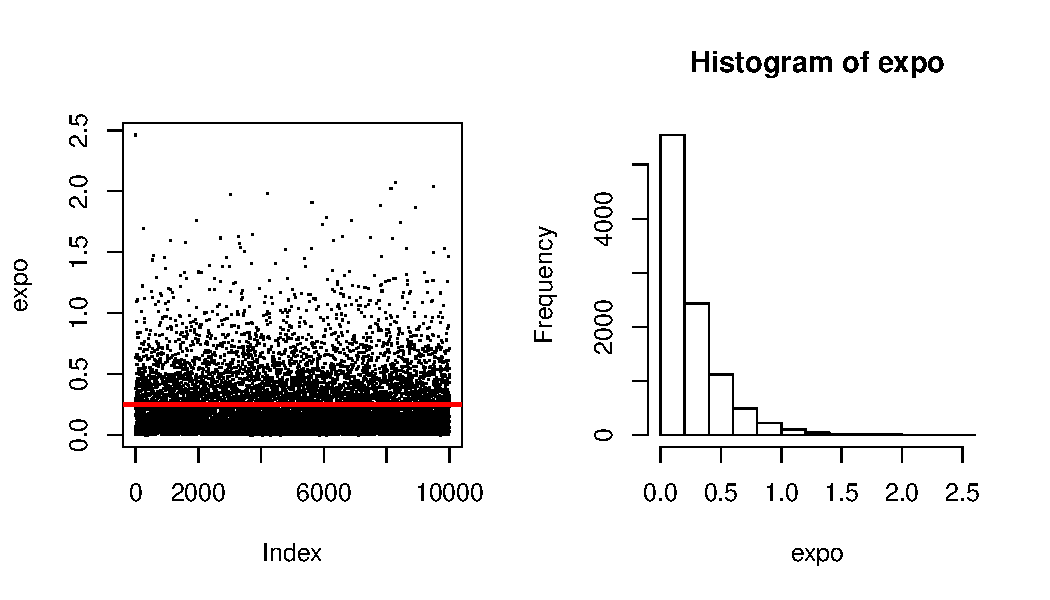
\includegraphics[width=.5\linewidth]{figure/RNG2} 
\begin{kframe}\begin{alltt}
\hlcom{## Normal}
\hlstd{norm} \hlkwb{<-} \hlkwd{rnorm}\hlstd{(}\hlkwc{n} \hlstd{=} \hlnum{10000}\hlstd{,} \hlkwc{mean} \hlstd{=} \hlnum{2.5}\hlstd{,} \hlkwc{sd} \hlstd{=} \hlnum{10}\hlstd{)}
\hlkwd{plot}\hlstd{(norm,} \hlkwc{pch} \hlstd{=} \hlstr{"."}\hlstd{)} \hlopt{+} \hlkwd{abline}\hlstd{(}\hlkwc{h} \hlstd{=} \hlkwd{mean}\hlstd{(norm),} \hlkwc{col} \hlstd{=} \hlnum{2}\hlstd{,} \hlkwc{lwd} \hlstd{=} \hlnum{3}\hlstd{)}
\hlkwd{hist}\hlstd{(norm)}
\end{alltt}
\end{kframe}
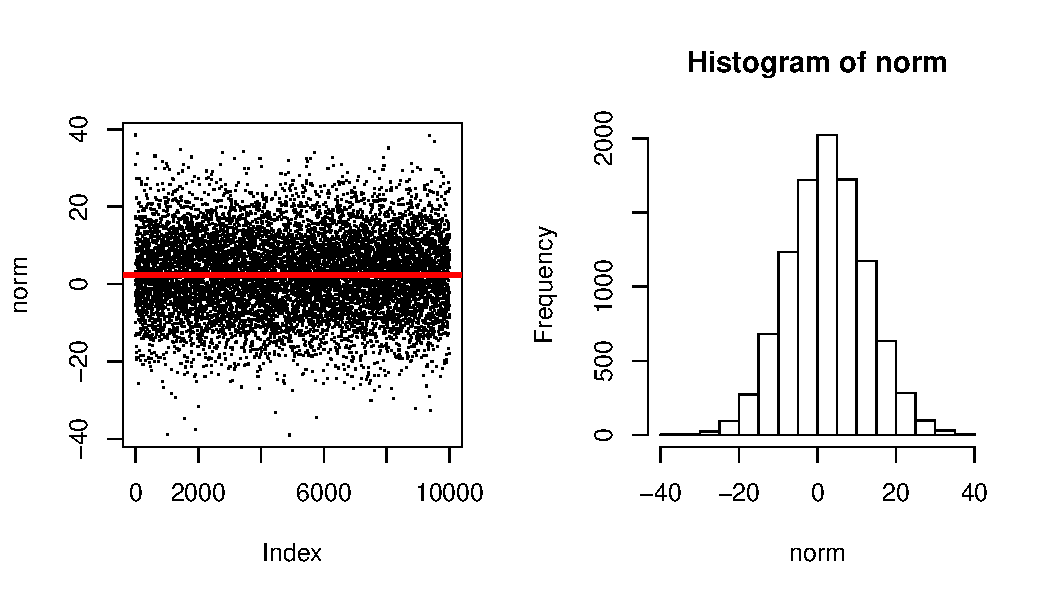
\includegraphics[width=.5\linewidth]{figure/RNG3} 
\begin{kframe}\begin{alltt}
\hlcom{## Poisson}
\hlstd{po} \hlkwb{<-} \hlkwd{rpois}\hlstd{(}\hlkwc{n} \hlstd{=} \hlnum{10000}\hlstd{,} \hlkwc{lambda} \hlstd{=} \hlnum{3.5}\hlstd{)}
\hlkwd{plot}\hlstd{(po)} \hlopt{+} \hlkwd{abline}\hlstd{(}\hlkwc{h} \hlstd{=} \hlkwd{mean}\hlstd{(po),} \hlkwc{col} \hlstd{=} \hlnum{2}\hlstd{,} \hlkwc{lwd} \hlstd{=} \hlnum{3}\hlstd{)}
\hlkwd{hist}\hlstd{(po)}
\end{alltt}
\end{kframe}
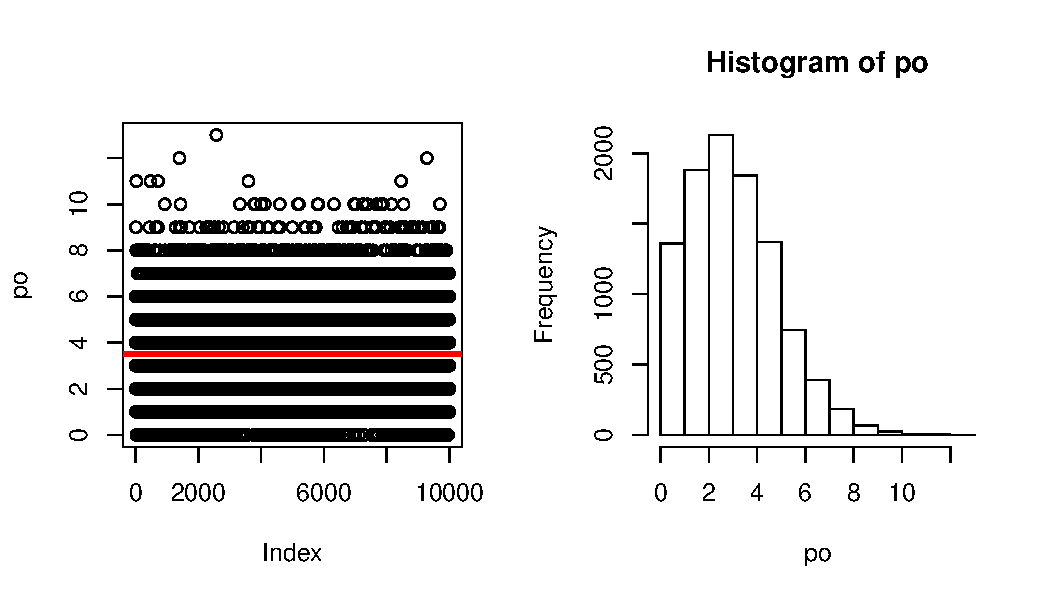
\includegraphics[width=.5\linewidth]{figure/RNG4} 

\end{knitrout}


\pagebreak
\bf{2.2 Binomial RNG and binomial from uniform RNG}
\begin{knitrout}
\definecolor{shadecolor}{rgb}{0.969, 0.969, 0.969}\color{fgcolor}\begin{kframe}
\begin{alltt}
\hlcom{## Binomial direct}
\hlkwd{layout}\hlstd{(}\hlkwd{matrix}\hlstd{(}\hlkwd{c}\hlstd{(}\hlnum{1}\hlstd{,} \hlnum{2}\hlstd{),} \hlnum{1}\hlstd{,} \hlnum{2}\hlstd{,} \hlkwc{byrow} \hlstd{=} \hlnum{TRUE}\hlstd{))}
\hlstd{bin} \hlkwb{<-} \hlkwd{rbinom}\hlstd{(}\hlkwc{n} \hlstd{=} \hlnum{100}\hlstd{,} \hlkwc{size} \hlstd{=} \hlnum{20}\hlstd{,} \hlkwc{prob} \hlstd{=} \hlnum{0.3}\hlstd{)}
\hlkwd{plot}\hlstd{(bin)} \hlopt{+} \hlkwd{abline}\hlstd{(}\hlkwc{h} \hlstd{=} \hlkwd{mean}\hlstd{(bin),} \hlkwc{col} \hlstd{=} \hlnum{2}\hlstd{,} \hlkwc{lwd} \hlstd{=} \hlnum{3}\hlstd{)}
\hlkwd{hist}\hlstd{(bin,} \hlkwc{breaks} \hlstd{=} \hlnum{0}\hlopt{:}\hlnum{20}\hlstd{)}
\end{alltt}
\end{kframe}
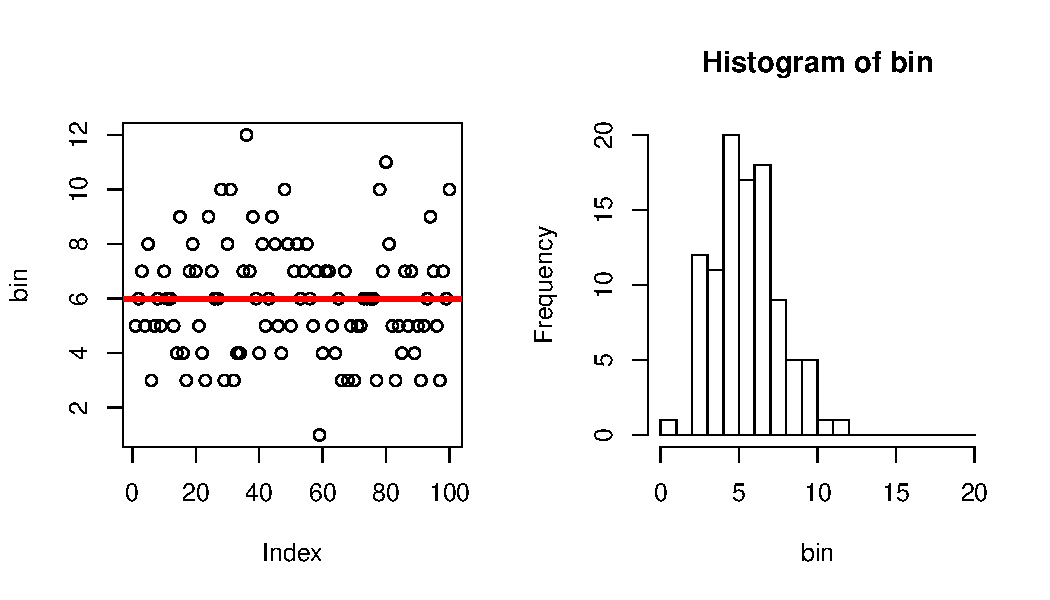
\includegraphics[width=.5\linewidth]{figure/bin1} 
\begin{kframe}\begin{alltt}
\hlcom{## Binomial from uniform}
\hlkwd{rm}\hlstd{(}\hlkwc{list} \hlstd{=} \hlkwd{ls}\hlstd{(}\hlkwc{all} \hlstd{=} \hlnum{TRUE}\hlstd{))}
\hlstd{all_ber} \hlkwb{<-} \hlkwa{NULL}
\hlkwa{for} \hlstd{(i} \hlkwa{in} \hlnum{1}\hlopt{:}\hlnum{20}\hlstd{) \{}
    \hlstd{unif} \hlkwb{<-} \hlkwd{runif}\hlstd{(}\hlkwc{n} \hlstd{=} \hlnum{100}\hlstd{,} \hlkwc{min} \hlstd{=} \hlnum{0}\hlstd{,} \hlkwc{max} \hlstd{=} \hlnum{1}\hlstd{)}
    \hlstd{ber} \hlkwb{<-} \hlkwd{ifelse}\hlstd{(unif} \hlopt{<} \hlnum{0.3}\hlstd{,} \hlnum{1}\hlstd{,} \hlnum{0}\hlstd{)}
    \hlstd{all_ber} \hlkwb{<-} \hlkwd{rbind}\hlstd{(all_ber, ber)}
\hlstd{\}}
\hlstd{bin} \hlkwb{<-} \hlkwd{colSums}\hlstd{(all_ber)}
\hlkwd{plot}\hlstd{(bin)} \hlopt{+} \hlkwd{abline}\hlstd{(}\hlkwc{h} \hlstd{=} \hlkwd{mean}\hlstd{(bin),} \hlkwc{col} \hlstd{=} \hlnum{2}\hlstd{,} \hlkwc{lwd} \hlstd{=} \hlnum{5}\hlstd{)}
\hlkwd{hist}\hlstd{(bin,} \hlkwc{breaks} \hlstd{=} \hlnum{0}\hlopt{:}\hlnum{20}\hlstd{)}
\end{alltt}
\end{kframe}
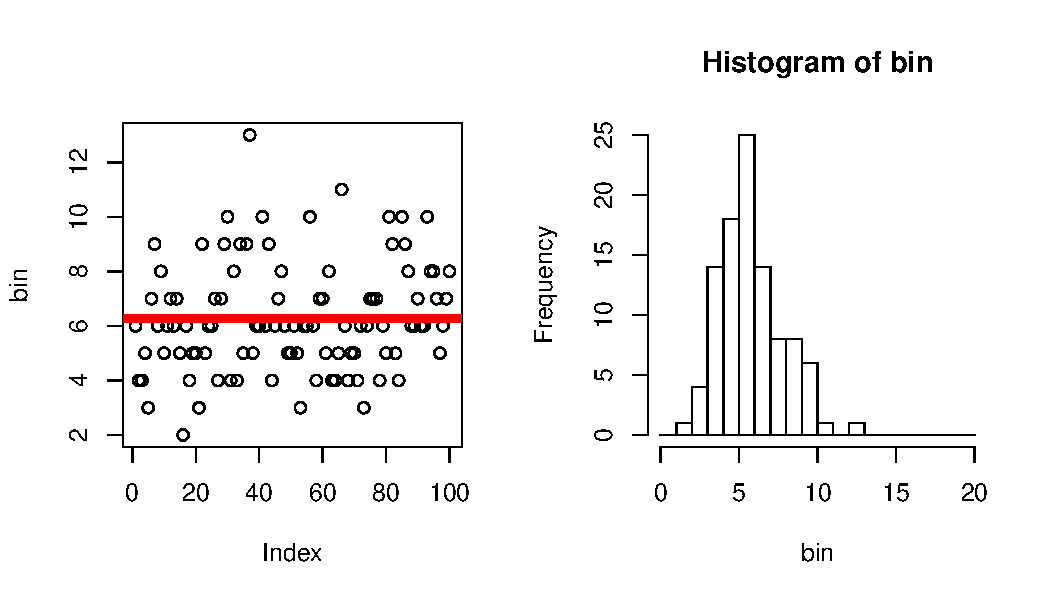
\includegraphics[width=.5\linewidth]{figure/bin2} 

\end{knitrout}


\pagebreak
\bf{2.3 RNG and time-steps}
\begin{knitrout}
\definecolor{shadecolor}{rgb}{0.969, 0.969, 0.969}\color{fgcolor}\begin{kframe}
\begin{alltt}
\hlkwd{rm}\hlstd{(}\hlkwc{list} \hlstd{=} \hlkwd{ls}\hlstd{(}\hlkwc{all} \hlstd{=} \hlnum{TRUE}\hlstd{))}
\hlkwd{layout}\hlstd{(}\hlkwd{matrix}\hlstd{(}\hlkwd{c}\hlstd{(}\hlnum{1}\hlopt{:}\hlnum{6}\hlstd{),} \hlnum{2}\hlstd{,} \hlnum{3}\hlstd{,} \hlkwc{byrow} \hlstd{=} \hlnum{TRUE}\hlstd{))}
\hlkwa{for} \hlstd{(dt} \hlkwa{in} \hlkwd{c}\hlstd{(}\hlnum{1}\hlstd{,} \hlnum{0.1}\hlstd{)) \{}
    \hlstd{derivs} \hlkwb{<-} \hlkwa{function}\hlstd{(}\hlkwc{times}\hlstd{,} \hlkwc{state}\hlstd{,} \hlkwc{parameters}\hlstd{) \{}
        \hlkwd{with}\hlstd{(}\hlkwd{as.list}\hlstd{(}\hlkwd{c}\hlstd{(state, parameters)), \{}
            \hlstd{dU} \hlkwb{<-} \hlstd{unif[times}\hlopt{/}\hlstd{dt]} \hlopt{-} \hlstd{c1} \hlopt{*} \hlstd{U}
            \hlstd{dUout} \hlkwb{<-} \hlstd{c1} \hlopt{*} \hlstd{U}
            \hlkwd{return}\hlstd{(}\hlkwd{list}\hlstd{(}\hlkwd{c}\hlstd{(dU, dUout)))}
        \hlstd{\})}
    \hlstd{\}}
    \hlstd{init} \hlkwb{<-} \hlkwd{c}\hlstd{(}\hlkwc{U} \hlstd{=} \hlnum{0}\hlstd{,} \hlkwc{Uout} \hlstd{=} \hlnum{0}\hlstd{)}
    \hlstd{times} \hlkwb{<-} \hlkwd{seq}\hlstd{(}\hlnum{1}\hlstd{,} \hlnum{100}\hlstd{,} \hlkwc{by} \hlstd{= dt)}
    \hlstd{unif} \hlkwb{<-} \hlkwd{runif}\hlstd{(}\hlkwc{n} \hlstd{=} \hlkwd{length}\hlstd{(times),} \hlkwc{min} \hlstd{=} \hlnum{0}\hlstd{,} \hlkwc{max} \hlstd{=} \hlnum{10}\hlstd{)}
    \hlstd{parameters} \hlkwb{<-} \hlkwd{c}\hlstd{(unif,} \hlkwc{c1} \hlstd{=} \hlnum{0.1}\hlstd{, dt)}
    \hlstd{out} \hlkwb{<-} \hlkwd{as.data.frame}\hlstd{(}\hlkwd{ode}\hlstd{(}\hlkwc{y} \hlstd{= init,} \hlkwc{times} \hlstd{= times,} \hlkwc{func} \hlstd{= derivs,} \hlkwc{parms} \hlstd{= parameters))}

    \hlcom{## Plot results}
    \hlkwd{plot}\hlstd{(times, unif,} \hlkwc{type} \hlstd{=} \hlstr{"l"}\hlstd{,} \hlkwc{xlab} \hlstd{=} \hlstr{"Time"}\hlstd{,} \hlkwc{ylab} \hlstd{=} \hlstr{"AU / t"}\hlstd{,} \hlkwc{main} \hlstd{=} \hlkwd{paste}\hlstd{(}\hlstr{"In_Unif, "}\hlstd{,}
        \hlkwd{sprintf}\hlstd{(}\hlstr{"dt=%.1f"}\hlstd{, dt)),} \hlkwc{lty} \hlstd{=} \hlnum{1}\hlstd{,} \hlkwc{bty} \hlstd{=} \hlstr{"l"}\hlstd{,} \hlkwc{col} \hlstd{=} \hlnum{2}\hlstd{)}
    \hlkwd{plot}\hlstd{(times, out}\hlopt{$}\hlstd{U,} \hlkwc{type} \hlstd{=} \hlstr{"l"}\hlstd{,} \hlkwc{xlab} \hlstd{=} \hlstr{"Time"}\hlstd{,} \hlkwc{ylab} \hlstd{=} \hlstr{"AU"}\hlstd{,} \hlkwc{main} \hlstd{=} \hlkwd{paste}\hlstd{(}\hlstr{"U, "}\hlstd{,}
        \hlkwd{sprintf}\hlstd{(}\hlstr{"dt=%.1f"}\hlstd{, dt)),} \hlkwc{lty} \hlstd{=} \hlnum{1}\hlstd{,} \hlkwc{bty} \hlstd{=} \hlstr{"l"}\hlstd{,} \hlkwc{col} \hlstd{=} \hlnum{2}\hlstd{)}
    \hlkwd{plot}\hlstd{(times, out}\hlopt{$}\hlstd{Uout}\hlopt{/}\hlstd{times,} \hlkwc{type} \hlstd{=} \hlstr{"l"}\hlstd{,} \hlkwc{xlab} \hlstd{=} \hlstr{"Time"}\hlstd{,} \hlkwc{ylab} \hlstd{=} \hlstr{"AU / t"}\hlstd{,}
        \hlkwc{main} \hlstd{=} \hlkwd{paste}\hlstd{(}\hlstr{"Out_U, "}\hlstd{,} \hlkwd{sprintf}\hlstd{(}\hlstr{"dt=%.1f"}\hlstd{, dt)),} \hlkwc{lty} \hlstd{=} \hlnum{1}\hlstd{,} \hlkwc{bty} \hlstd{=} \hlstr{"l"}\hlstd{,}
        \hlkwc{col} \hlstd{=} \hlnum{2}\hlstd{)}
\hlstd{\}}
\end{alltt}
\end{kframe}
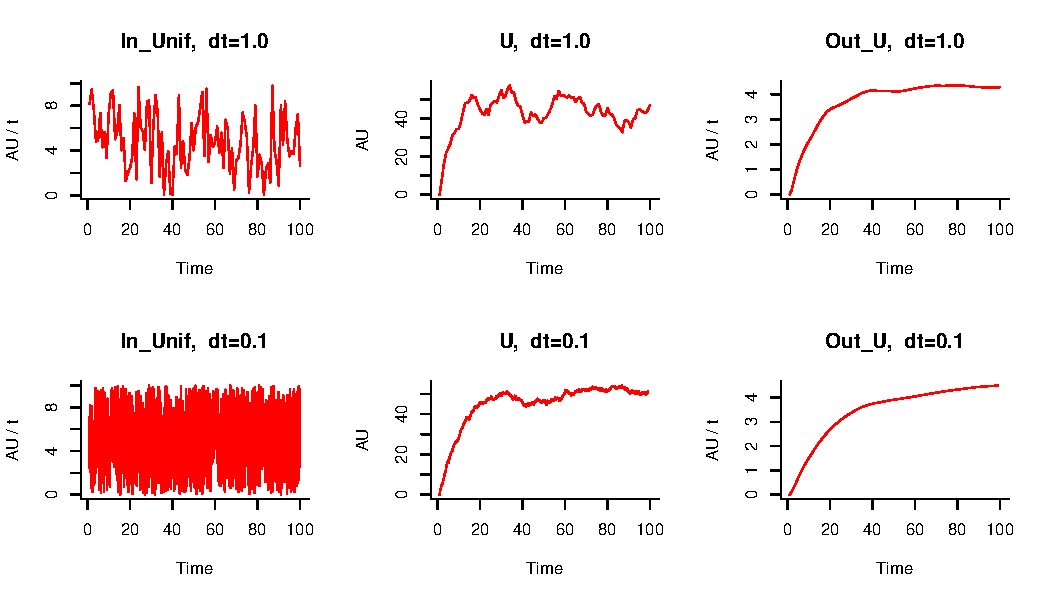
\includegraphics[width=.5\linewidth]{figure/time_step} 

\end{knitrout}

\pagebreak
\bf{2.4 Seeds - making a stochastic simulation reproducible}
\begin{knitrout}
\definecolor{shadecolor}{rgb}{0.969, 0.969, 0.969}\color{fgcolor}\begin{kframe}
\begin{alltt}
\hlkwd{rm}\hlstd{(}\hlkwc{list} \hlstd{=} \hlkwd{ls}\hlstd{(}\hlkwc{all} \hlstd{=} \hlnum{TRUE}\hlstd{))}
\hlkwd{layout}\hlstd{(}\hlkwd{matrix}\hlstd{(}\hlkwd{c}\hlstd{(}\hlnum{1}\hlopt{:}\hlnum{2}\hlstd{),} \hlnum{1}\hlstd{,} \hlnum{2}\hlstd{,} \hlkwc{byrow} \hlstd{=} \hlnum{TRUE}\hlstd{))}
\hlkwd{set.seed}\hlstd{(}\hlnum{1234}\hlstd{)}
\hlstd{un1} \hlkwb{<-} \hlkwd{runif}\hlstd{(}\hlkwc{n} \hlstd{=} \hlnum{100}\hlstd{,} \hlkwc{min} \hlstd{=} \hlnum{0}\hlstd{,} \hlkwc{max} \hlstd{=} \hlnum{10}\hlstd{)}
\hlkwd{set.seed}\hlstd{(}\hlnum{1234}\hlstd{)}
\hlstd{un2} \hlkwb{<-} \hlkwd{runif}\hlstd{(}\hlkwc{n} \hlstd{=} \hlnum{100}\hlstd{,} \hlkwc{min} \hlstd{=} \hlnum{0}\hlstd{,} \hlkwc{max} \hlstd{=} \hlnum{10}\hlstd{)}
\hlkwd{plot}\hlstd{(}\hlnum{1}\hlopt{:}\hlnum{100}\hlstd{, un1,} \hlkwc{type} \hlstd{=} \hlstr{"l"}\hlstd{,} \hlkwc{xlab} \hlstd{=} \hlstr{"Time"}\hlstd{,} \hlkwc{ylab} \hlstd{=} \hlstr{"AU"}\hlstd{,} \hlkwc{main} \hlstd{=} \hlstr{"Uniform 1"}\hlstd{,}
    \hlkwc{lty} \hlstd{=} \hlnum{1}\hlstd{,} \hlkwc{bty} \hlstd{=} \hlstr{"l"}\hlstd{,} \hlkwc{col} \hlstd{=} \hlnum{2}\hlstd{)}
\hlkwd{plot}\hlstd{(}\hlnum{1}\hlopt{:}\hlnum{100}\hlstd{, un2,} \hlkwc{type} \hlstd{=} \hlstr{"l"}\hlstd{,} \hlkwc{xlab} \hlstd{=} \hlstr{"Time"}\hlstd{,} \hlkwc{ylab} \hlstd{=} \hlstr{"AU"}\hlstd{,} \hlkwc{main} \hlstd{=} \hlstr{"Uniform 2"}\hlstd{,}
    \hlkwc{lty} \hlstd{=} \hlnum{1}\hlstd{,} \hlkwc{bty} \hlstd{=} \hlstr{"l"}\hlstd{,} \hlkwc{col} \hlstd{=} \hlnum{2}\hlstd{)}
\end{alltt}
\end{kframe}
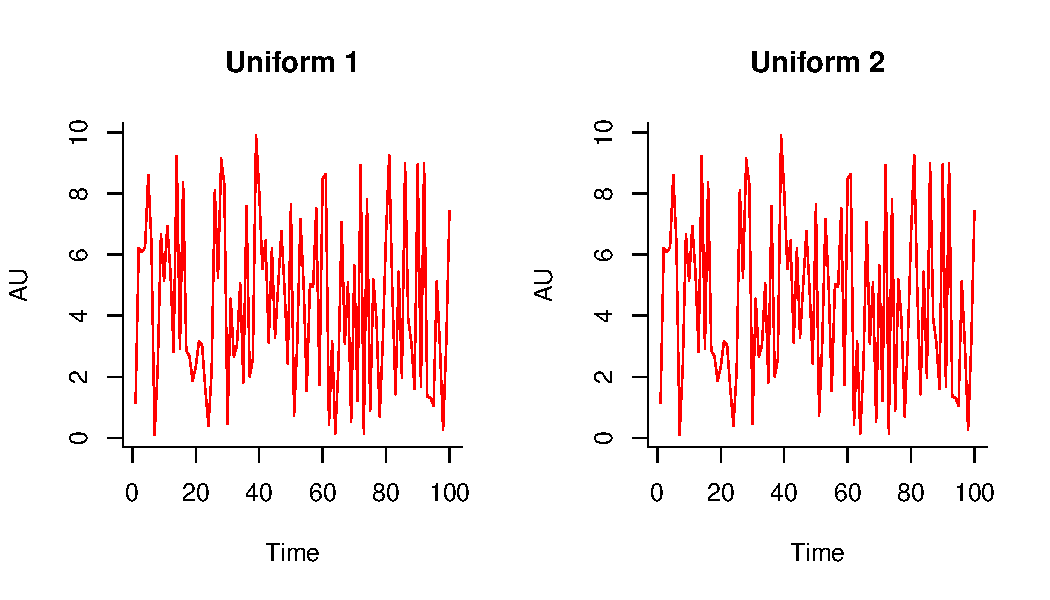
\includegraphics[width=.5\linewidth]{figure/seeds} 

\end{knitrout}


\bf{3.1 Demographic Stochasticity}
\begin{knitrout}
\definecolor{shadecolor}{rgb}{0.969, 0.969, 0.969}\color{fgcolor}\begin{kframe}
\begin{alltt}
\hlkwd{rm}\hlstd{(}\hlkwc{list} \hlstd{=} \hlkwd{ls}\hlstd{(}\hlkwc{all} \hlstd{=} \hlnum{TRUE}\hlstd{))}
\hlkwd{layout}\hlstd{(}\hlkwd{matrix}\hlstd{(}\hlnum{1}\hlopt{:}\hlnum{2}\hlstd{,} \hlnum{1}\hlstd{,} \hlnum{2}\hlstd{))}
\hlstd{init} \hlkwb{<-} \hlkwd{c}\hlstd{(}\hlkwc{X} \hlstd{=} \hlnum{1}\hlstd{)}
\hlstd{parms} \hlkwb{<-} \hlkwd{c}\hlstd{(}\hlkwc{c1} \hlstd{=} \hlnum{1}\hlstd{,} \hlkwc{c2} \hlstd{=} \hlnum{0.01}\hlstd{)}
\hlstd{deriv} \hlkwb{<-} \hlkwa{function}\hlstd{(}\hlkwc{times}\hlstd{,} \hlkwc{state}\hlstd{,} \hlkwc{parameters}\hlstd{) \{}
    \hlkwd{with}\hlstd{(}\hlkwd{as.list}\hlstd{(}\hlkwd{c}\hlstd{(state, parameters)), \{}
        \hlstd{dX} \hlkwb{<-} \hlstd{c1} \hlopt{*} \hlstd{X} \hlopt{-} \hlstd{c2} \hlopt{*} \hlstd{X} \hlopt{*} \hlstd{X}
        \hlkwd{return}\hlstd{(}\hlkwd{list}\hlstd{(}\hlkwd{c}\hlstd{(dX)))}
    \hlstd{\})}
\hlstd{\}}
\hlstd{times} \hlkwb{<-} \hlkwd{seq}\hlstd{(}\hlnum{0}\hlstd{,} \hlnum{20}\hlstd{,} \hlkwc{by} \hlstd{=} \hlnum{0.01}\hlstd{)}
\hlstd{out} \hlkwb{<-} \hlkwd{as.data.frame}\hlstd{(}\hlkwd{ode}\hlstd{(}\hlkwc{y} \hlstd{= init,} \hlkwc{times} \hlstd{= times,} \hlkwc{func} \hlstd{= deriv,} \hlkwc{parms} \hlstd{= parms))}
\hlstd{out}\hlopt{$}\hlstd{time} \hlkwb{<-} \hlkwa{NULL}
\hlkwd{matplot}\hlstd{(times, out,} \hlkwc{type} \hlstd{=} \hlstr{"l"}\hlstd{,} \hlkwc{xlab} \hlstd{=} \hlstr{"Time"}\hlstd{,} \hlkwc{ylab} \hlstd{=} \hlstr{"AU"}\hlstd{,} \hlkwc{ylim} \hlstd{=} \hlkwd{c}\hlstd{(}\hlnum{0}\hlstd{,} \hlnum{120}\hlstd{),}
    \hlkwc{main} \hlstd{=} \hlstr{"Deterministic Logistic Model"}\hlstd{,} \hlkwc{lty} \hlstd{=} \hlnum{1}\hlstd{,} \hlkwc{lwd} \hlstd{=} \hlnum{1}\hlstd{,} \hlkwc{col} \hlstd{=} \hlnum{2}\hlstd{)}
\hlstd{a} \hlkwb{<-} \hlkwd{c}\hlstd{(}\hlstr{"c1 * X"}\hlstd{,} \hlstr{"c2 * X * X"}\hlstd{)}
\hlstd{nu} \hlkwb{<-} \hlkwd{matrix}\hlstd{(}\hlkwd{c}\hlstd{(}\hlopt{+}\hlnum{1}\hlstd{,} \hlopt{-}\hlnum{1}\hlstd{),} \hlkwc{ncol} \hlstd{=} \hlnum{2}\hlstd{)}
\hlstd{out} \hlkwb{<-} \hlkwd{ssa}\hlstd{(init, a, nu, parms,} \hlkwc{tf} \hlstd{=} \hlnum{20}\hlstd{,} \hlkwc{tau} \hlstd{=} \hlnum{0.01}\hlstd{,} \hlkwc{method} \hlstd{=} \hlstr{"ETL"}\hlstd{,} \hlkwc{maxWallTime} \hlstd{=} \hlnum{5}\hlstd{,}
    \hlkwc{simName} \hlstd{=} \hlstr{"Stochastic Logistic Model"}\hlstd{)}
\hlcom{#'Explicit tau-leap' => user-defined step size}
\hlkwd{ssa.plot}\hlstd{(out,} \hlkwc{show.legend} \hlstd{= F)}
\end{alltt}
\end{kframe}
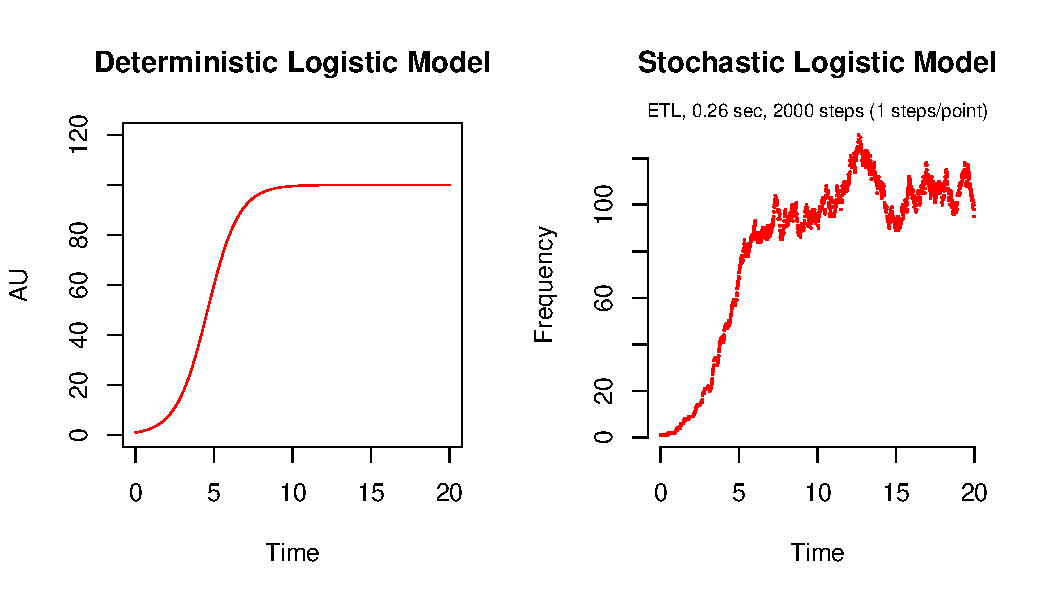
\includegraphics[width=.5\linewidth]{figure/demographic} 

\end{knitrout}


\bf{3.2 Environmental Stochasticity}
\begin{knitrout}
\definecolor{shadecolor}{rgb}{0.969, 0.969, 0.969}\color{fgcolor}\begin{kframe}
\begin{alltt}
\hlkwd{rm}\hlstd{(}\hlkwc{list} \hlstd{=} \hlkwd{ls}\hlstd{(}\hlkwc{all} \hlstd{=} \hlnum{TRUE}\hlstd{))}
\hlkwd{layout}\hlstd{(}\hlkwd{matrix}\hlstd{(}\hlnum{1}\hlopt{:}\hlnum{2}\hlstd{,} \hlnum{1}\hlstd{,} \hlnum{2}\hlstd{))}
\hlkwa{for} \hlstd{(f} \hlkwa{in} \hlkwd{c}\hlstd{(}\hlnum{5}\hlstd{,} \hlnum{0.1}\hlstd{)) \{}
    \hlstd{deriv} \hlkwb{<-} \hlkwa{function}\hlstd{(}\hlkwc{Time}\hlstd{,} \hlkwc{state}\hlstd{,} \hlkwc{parameters}\hlstd{) \{}
        \hlkwd{with}\hlstd{(}\hlkwd{as.list}\hlstd{(}\hlkwd{c}\hlstd{(state, parameters)), \{}
            \hlkwd{set.seed}\hlstd{(}\hlnum{1000} \hlopt{+} \hlkwd{ceiling}\hlstd{(Time}\hlopt{/}\hlstd{f))}  \hlcom{#Shifting seed at an interval}
            \hlstd{c1} \hlkwb{<-} \hlkwd{runif}\hlstd{(}\hlnum{1}\hlstd{,} \hlnum{0.5} \hlopt{*} \hlstd{c1,} \hlnum{1.5} \hlopt{*} \hlstd{c1)}
            \hlkwd{set.seed}\hlstd{(}\hlnum{2000} \hlopt{+} \hlkwd{ceiling}\hlstd{(Time}\hlopt{/}\hlstd{f))}
            \hlstd{c2} \hlkwb{<-} \hlkwd{rnorm}\hlstd{(}\hlnum{1}\hlstd{, c2,} \hlnum{0.2} \hlopt{*} \hlstd{c2)}
            \hlstd{dX} \hlkwb{<-} \hlstd{c1} \hlopt{*} \hlstd{X} \hlopt{-} \hlstd{c2} \hlopt{*} \hlstd{X} \hlopt{*} \hlstd{X}
            \hlkwd{return}\hlstd{(}\hlkwd{list}\hlstd{(}\hlkwd{c}\hlstd{(dX)))}
        \hlstd{\})}
    \hlstd{\}}
    \hlstd{init} \hlkwb{<-} \hlkwd{c}\hlstd{(}\hlkwc{X} \hlstd{=} \hlnum{1}\hlstd{)}
    \hlstd{times} \hlkwb{<-} \hlkwd{seq}\hlstd{(}\hlnum{0}\hlstd{,} \hlnum{20}\hlstd{,} \hlkwc{by} \hlstd{=} \hlnum{0.01}\hlstd{)}
    \hlstd{parameters} \hlkwb{<-} \hlkwd{c}\hlstd{(}\hlkwc{c1} \hlstd{=} \hlnum{1}\hlstd{,} \hlkwc{c2} \hlstd{=} \hlnum{0.01}\hlstd{, f)}
    \hlstd{out} \hlkwb{<-} \hlkwd{as.data.frame}\hlstd{(}\hlkwd{ode}\hlstd{(}\hlkwc{y} \hlstd{= init,} \hlkwc{times} \hlstd{= times,} \hlkwc{func} \hlstd{= deriv,} \hlkwc{parms} \hlstd{= parameters))}
    \hlstd{out}\hlopt{$}\hlstd{time} \hlkwb{<-} \hlkwa{NULL}
    \hlkwd{matplot}\hlstd{(times, out,} \hlkwc{type} \hlstd{=} \hlstr{"l"}\hlstd{,} \hlkwc{xlab} \hlstd{=} \hlstr{"Time"}\hlstd{,} \hlkwc{ylab} \hlstd{=} \hlstr{"AU"}\hlstd{,} \hlkwc{ylim} \hlstd{=} \hlkwd{c}\hlstd{(}\hlnum{0}\hlstd{,}
        \hlnum{120}\hlstd{),} \hlkwc{main} \hlstd{=} \hlkwd{paste}\hlstd{(}\hlstr{"Environmental Stochasticity\textbackslash{}n"}\hlstd{,} \hlkwd{sprintf}\hlstd{(}\hlstr{"Interval=%.1f"}\hlstd{,}
        \hlstd{f)),} \hlkwc{lty} \hlstd{=} \hlnum{1}\hlstd{,} \hlkwc{lwd} \hlstd{=} \hlnum{1}\hlstd{,} \hlkwc{col} \hlstd{=} \hlnum{2}\hlstd{)}
\hlstd{\}}
\end{alltt}
\end{kframe}
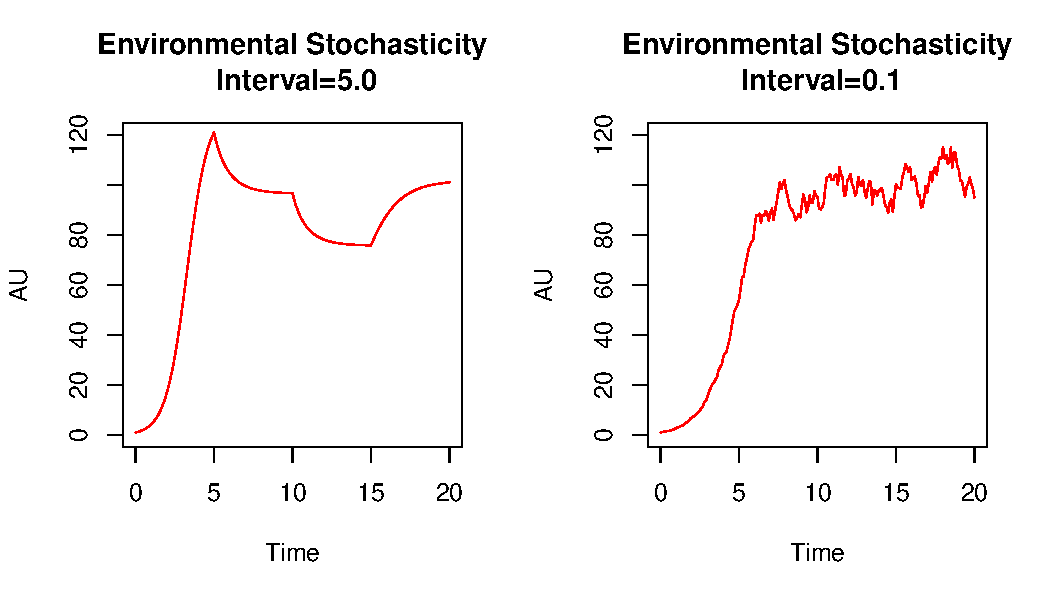
\includegraphics[width=.5\linewidth]{figure/environmental} 

\end{knitrout}


\bf{3.3 Initial Value Stochasticity}
\begin{knitrout}
\definecolor{shadecolor}{rgb}{0.969, 0.969, 0.969}\color{fgcolor}\begin{kframe}
\begin{alltt}
\hlkwd{rm}\hlstd{(}\hlkwc{list} \hlstd{=} \hlkwd{ls}\hlstd{(}\hlkwc{all} \hlstd{=} \hlnum{TRUE}\hlstd{))}
\hlkwd{layout}\hlstd{(}\hlkwd{matrix}\hlstd{(}\hlnum{1}\hlopt{:}\hlnum{2}\hlstd{,} \hlnum{1}\hlstd{,} \hlnum{2}\hlstd{))}
\hlkwa{for} \hlstd{(seed_n} \hlkwa{in} \hlkwd{c}\hlstd{(}\hlnum{1}\hlstd{,} \hlnum{1000}\hlstd{)) \{}
    \hlkwd{set.seed}\hlstd{(seed_n)}
    \hlstd{deriv} \hlkwb{<-} \hlkwa{function}\hlstd{(}\hlkwc{Time}\hlstd{,} \hlkwc{state}\hlstd{,} \hlkwc{parameters}\hlstd{) \{}
        \hlkwd{with}\hlstd{(}\hlkwd{as.list}\hlstd{(}\hlkwd{c}\hlstd{(state, parameters)), \{}
            \hlstd{dX} \hlkwb{<-} \hlstd{c1} \hlopt{*} \hlstd{X} \hlopt{-} \hlstd{c2} \hlopt{*} \hlstd{X} \hlopt{*} \hlstd{X}
            \hlkwd{return}\hlstd{(}\hlkwd{list}\hlstd{(}\hlkwd{c}\hlstd{(dX)))}
        \hlstd{\})}
    \hlstd{\}}
    \hlstd{init} \hlkwb{<-} \hlkwd{c}\hlstd{(}\hlkwc{X} \hlstd{=} \hlkwd{rbinom}\hlstd{(}\hlnum{1}\hlstd{,} \hlnum{5}\hlstd{,} \hlnum{0.2}\hlstd{))}
    \hlstd{times} \hlkwb{<-} \hlkwd{seq}\hlstd{(}\hlnum{0}\hlstd{,} \hlnum{20}\hlstd{,} \hlkwc{by} \hlstd{=} \hlnum{0.01}\hlstd{)}
    \hlstd{parameters} \hlkwb{<-} \hlkwd{c}\hlstd{(}\hlkwc{c1} \hlstd{=} \hlnum{1}\hlstd{,} \hlkwc{c2} \hlstd{=} \hlnum{0.01}\hlstd{)}
    \hlstd{out} \hlkwb{<-} \hlkwd{as.data.frame}\hlstd{(}\hlkwd{ode}\hlstd{(}\hlkwc{y} \hlstd{= init,} \hlkwc{times} \hlstd{= times,} \hlkwc{func} \hlstd{= deriv,} \hlkwc{parms} \hlstd{= parameters))}
    \hlstd{out}\hlopt{$}\hlstd{time} \hlkwb{<-} \hlkwa{NULL}
    \hlkwd{matplot}\hlstd{(times, out,} \hlkwc{type} \hlstd{=} \hlstr{"l"}\hlstd{,} \hlkwc{xlab} \hlstd{=} \hlstr{"Time"}\hlstd{,} \hlkwc{ylab} \hlstd{=} \hlstr{"AU"}\hlstd{,} \hlkwc{ylim} \hlstd{=} \hlkwd{c}\hlstd{(}\hlnum{0}\hlstd{,}
        \hlnum{120}\hlstd{),} \hlkwc{main} \hlstd{=} \hlstr{"Initial Value Stochasticity"}\hlstd{,} \hlkwc{lty} \hlstd{=} \hlnum{1}\hlstd{,} \hlkwc{lwd} \hlstd{=} \hlnum{1}\hlstd{,} \hlkwc{col} \hlstd{=} \hlnum{2}\hlstd{)}
\hlstd{\}}
\end{alltt}
\end{kframe}
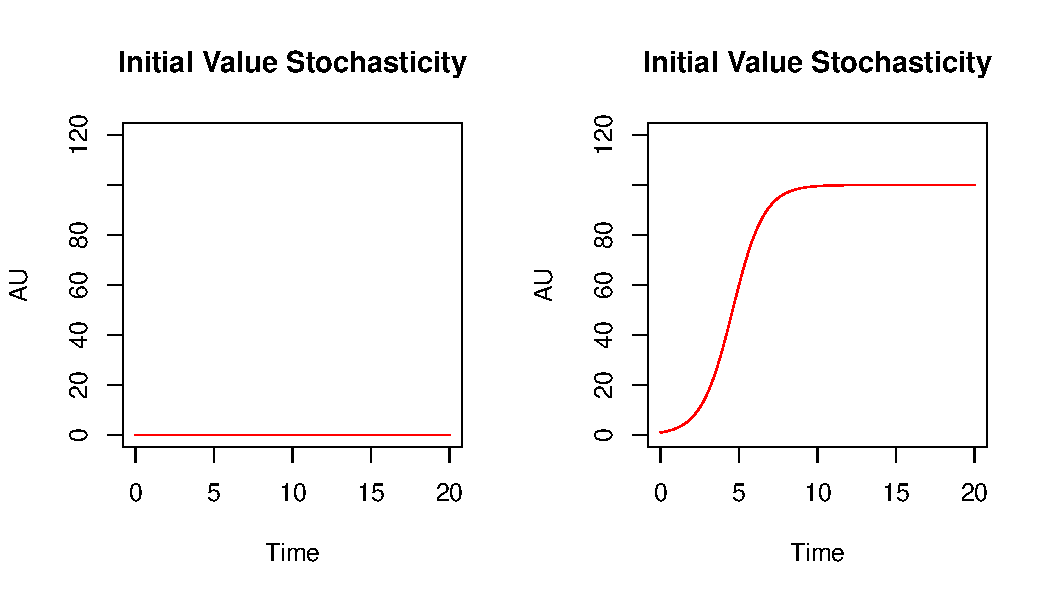
\includegraphics[width=.5\linewidth]{figure/initial} 

\end{knitrout}


\bf{4.1 Output within replication}
\begin{knitrout}
\definecolor{shadecolor}{rgb}{0.969, 0.969, 0.969}\color{fgcolor}\begin{kframe}
\begin{alltt}
\hlkwd{rm}\hlstd{(}\hlkwc{list} \hlstd{=} \hlkwd{ls}\hlstd{(}\hlkwc{all} \hlstd{=} \hlnum{TRUE}\hlstd{))}
\hlkwd{layout}\hlstd{(}\hlkwd{matrix}\hlstd{(}\hlnum{1}\hlopt{:}\hlnum{2}\hlstd{,} \hlnum{1}\hlstd{,} \hlnum{2}\hlstd{))}
\hlstd{parms} \hlkwb{<-} \hlkwd{c}\hlstd{(}\hlkwc{c1} \hlstd{=} \hlnum{1}\hlstd{,} \hlkwc{c2} \hlstd{=} \hlnum{0.01}\hlstd{)}
\hlstd{x0} \hlkwb{<-} \hlkwd{c}\hlstd{(}\hlkwc{X} \hlstd{=} \hlnum{100}\hlstd{)}
\hlstd{a} \hlkwb{<-} \hlkwd{c}\hlstd{(}\hlstr{"c1 * X"}\hlstd{,} \hlstr{"c2 * X * X"}\hlstd{)}
\hlstd{nu} \hlkwb{<-} \hlkwd{matrix}\hlstd{(}\hlkwd{c}\hlstd{(}\hlopt{+}\hlnum{1}\hlstd{,} \hlopt{-}\hlnum{1}\hlstd{),} \hlkwc{ncol} \hlstd{=} \hlnum{2}\hlstd{)}
\hlstd{sim_out} \hlkwb{<-} \hlkwd{data.frame}\hlstd{(}\hlkwc{dt} \hlstd{=} \hlkwd{character}\hlstd{(),} \hlkwc{X} \hlstd{=} \hlkwd{numeric}\hlstd{())}
\hlkwa{for} \hlstd{(dt} \hlkwa{in} \hlkwd{c}\hlstd{(}\hlnum{0.1}\hlstd{,} \hlnum{0.01}\hlstd{)) \{}
    \hlstd{out} \hlkwb{<-} \hlkwd{ssa}\hlstd{(x0, a, nu, parms,} \hlkwc{tf} \hlstd{=} \hlnum{100}\hlstd{,} \hlkwc{tau} \hlstd{= dt,} \hlkwc{method} \hlstd{=} \hlstr{"ETL"}\hlstd{,} \hlkwc{maxWallTime} \hlstd{=} \hlnum{5}\hlstd{,}
        \hlkwc{simName} \hlstd{=} \hlstr{"Stochastic Logistic Model"}\hlstd{)}
    \hlcom{#'Explicit tau-leap' => user-defined step size}

    \hlcom{## Plot results}
    \hlkwd{ssa.plot}\hlstd{(out,} \hlkwc{show.legend} \hlstd{= F)} \hlopt{+} \hlkwd{abline}\hlstd{(}\hlkwc{h} \hlstd{=} \hlkwd{mean}\hlstd{(out}\hlopt{$}\hlstd{data[,} \hlnum{2}\hlstd{]),} \hlkwc{col} \hlstd{=} \hlnum{1}\hlstd{)} \hlopt{+}
        \hlkwd{abline}\hlstd{(}\hlkwc{h} \hlstd{=} \hlkwd{mean}\hlstd{(out}\hlopt{$}\hlstd{data[,} \hlnum{2}\hlstd{])} \hlopt{+} \hlkwd{sd}\hlstd{(out}\hlopt{$}\hlstd{data[,} \hlnum{2}\hlstd{]),} \hlkwc{col} \hlstd{=} \hlnum{1}\hlstd{,} \hlkwc{lty} \hlstd{=} \hlnum{3}\hlstd{)} \hlopt{+}
        \hlkwd{abline}\hlstd{(}\hlkwc{h} \hlstd{=} \hlkwd{mean}\hlstd{(out}\hlopt{$}\hlstd{data[,} \hlnum{2}\hlstd{])} \hlopt{-} \hlkwd{sd}\hlstd{(out}\hlopt{$}\hlstd{data[,} \hlnum{2}\hlstd{]),} \hlkwc{col} \hlstd{=} \hlnum{1}\hlstd{,} \hlkwc{lty} \hlstd{=} \hlnum{3}\hlstd{)}
    \hlstd{sim_out} \hlkwb{<-} \hlkwd{rbind}\hlstd{(sim_out,} \hlkwd{data.frame}\hlstd{(}\hlkwc{dt} \hlstd{=} \hlkwd{rep}\hlstd{(dt,} \hlkwd{nrow}\hlstd{(out}\hlopt{$}\hlstd{data)),} \hlkwc{X} \hlstd{= out}\hlopt{$}\hlstd{data[,}
        \hlnum{2}\hlstd{]))}
\hlstd{\}}
\end{alltt}
\end{kframe}
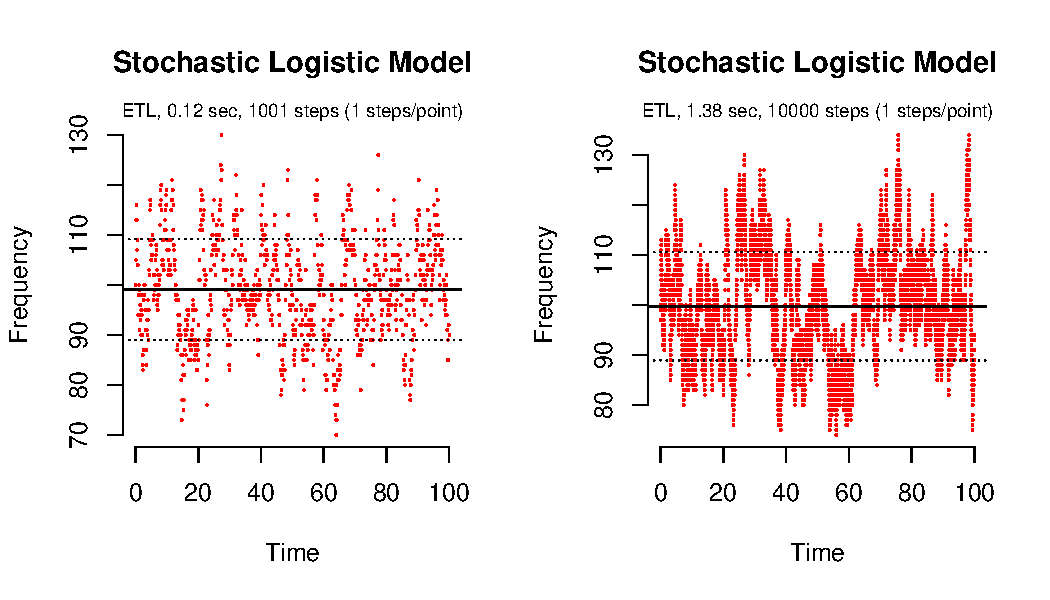
\includegraphics[width=.5\linewidth]{figure/within} 

\end{knitrout}


Within replication summary:
\begin{knitrout}
\definecolor{shadecolor}{rgb}{0.969, 0.969, 0.969}\color{fgcolor}\begin{kframe}
\begin{alltt}
\hlstd{dt_summay} \hlkwb{<-} \hlkwd{ddply}\hlstd{(sim_out,} \hlkwd{.}\hlstd{(dt), summarise,} \hlkwc{Lowest_X} \hlstd{=} \hlkwd{min}\hlstd{(X),} \hlkwc{Highest_X} \hlstd{=} \hlkwd{max}\hlstd{(X),}
    \hlkwc{StdDev_X} \hlstd{=} \hlkwd{round}\hlstd{(}\hlkwd{sd}\hlstd{(X),} \hlnum{0}\hlstd{))}
\hlkwd{print}\hlstd{(dt_summay)}
\end{alltt}
\begin{verbatim}
    dt Lowest_X Highest_X StdDev_X
1 0.01       74       134       11
2 0.10       70       130       10
\end{verbatim}
\end{kframe}
\end{knitrout}


\bf{4.2 Output over many replications}
\begin{knitrout}
\definecolor{shadecolor}{rgb}{0.969, 0.969, 0.969}\color{fgcolor}\begin{kframe}
\begin{alltt}
\hlkwd{rm}\hlstd{(}\hlkwc{list} \hlstd{=} \hlkwd{ls}\hlstd{(}\hlkwc{all} \hlstd{=} \hlnum{TRUE}\hlstd{))}
\hlstd{sim_out} \hlkwb{<-} \hlkwd{data.frame}\hlstd{(}\hlkwc{Repetition} \hlstd{=} \hlkwd{numeric}\hlstd{(),} \hlkwc{Sample} \hlstd{=} \hlkwd{numeric}\hlstd{(),} \hlkwc{Time} \hlstd{=} \hlkwd{double}\hlstd{(),}
    \hlkwc{X} \hlstd{=} \hlkwd{double}\hlstd{())}
\hlstd{parms} \hlkwb{<-} \hlkwd{c}\hlstd{(}\hlkwc{c1} \hlstd{=} \hlnum{1}\hlstd{,} \hlkwc{c2} \hlstd{=} \hlnum{0.01}\hlstd{)}
\hlstd{x0} \hlkwb{<-} \hlkwd{c}\hlstd{(}\hlkwc{X} \hlstd{=} \hlnum{100}\hlstd{)}
\hlstd{a} \hlkwb{<-} \hlkwd{c}\hlstd{(}\hlstr{"c1 * X"}\hlstd{,} \hlstr{"c2 * X * X"}\hlstd{)}
\hlstd{nu} \hlkwb{<-} \hlkwd{matrix}\hlstd{(}\hlkwd{c}\hlstd{(}\hlopt{+}\hlnum{1}\hlstd{,} \hlopt{-}\hlnum{1}\hlstd{),} \hlkwc{ncol} \hlstd{=} \hlnum{2}\hlstd{)}
\hlkwa{for} \hlstd{(i} \hlkwa{in} \hlkwd{c}\hlstd{(}\hlnum{1}\hlopt{:}\hlnum{10}\hlstd{)) \{}
    \hlstd{out} \hlkwb{<-} \hlkwd{ssa}\hlstd{(x0, a, nu, parms,} \hlkwc{tf} \hlstd{=} \hlnum{100}\hlstd{,} \hlkwc{tau} \hlstd{=} \hlnum{1}\hlstd{,} \hlkwc{method} \hlstd{=} \hlstr{"ETL"}\hlstd{,} \hlkwc{maxWallTime} \hlstd{=} \hlnum{5}\hlstd{)}
    \hlcom{#'Explicit tau-leap' => user-defined step size}
    \hlkwd{colnames}\hlstd{(out}\hlopt{$}\hlstd{data)[}\hlnum{1}\hlstd{]} \hlkwb{<-} \hlstr{"Time"}
    \hlstd{Repetition} \hlkwb{<-} \hlkwd{rep}\hlstd{(i,} \hlkwd{nrow}\hlstd{(out}\hlopt{$}\hlstd{data))}
    \hlstd{Sample} \hlkwb{<-} \hlnum{1}\hlopt{:}\hlkwd{nrow}\hlstd{(out}\hlopt{$}\hlstd{data)}
    \hlstd{sim_out} \hlkwb{<-} \hlkwd{rbind}\hlstd{(sim_out,} \hlkwd{cbind}\hlstd{(Repetition, Sample, out}\hlopt{$}\hlstd{data))}
\hlstd{\}}
\hlstd{within_summary} \hlkwb{<-} \hlkwd{ddply}\hlstd{(sim_out,} \hlkwd{.}\hlstd{(Repetition), summarise,} \hlkwc{X_end} \hlstd{=} \hlkwd{tail}\hlstd{(X,} \hlkwc{n} \hlstd{=} \hlnum{1}\hlstd{),}
    \hlkwc{X_max} \hlstd{=} \hlkwd{max}\hlstd{(X))}

\hlcom{## Plot results}
\hlkwd{ggplot}\hlstd{(}\hlkwc{data} \hlstd{= sim_out,} \hlkwd{aes}\hlstd{(}\hlkwc{x} \hlstd{= Time,} \hlkwc{y} \hlstd{= X,} \hlkwc{colour} \hlstd{= Repetition))} \hlopt{+} \hlkwd{geom_line}\hlstd{(}\hlkwd{aes}\hlstd{(}\hlkwc{group} \hlstd{= Repetition))}
\end{alltt}
\end{kframe}
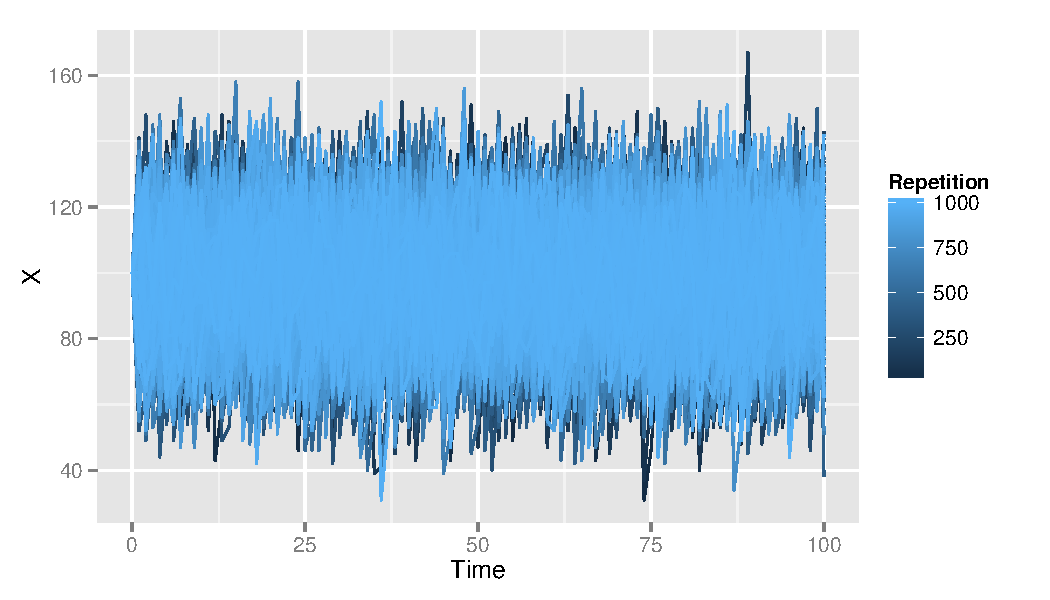
\includegraphics[width=.8\linewidth]{figure/many1} 
\begin{kframe}\begin{alltt}
\hlstd{median_quantiles} \hlkwb{<-} \hlkwd{quantile}\hlstd{(within_summary}\hlopt{$}\hlstd{X_end,} \hlkwd{c}\hlstd{(}\hlnum{0.025}\hlstd{,} \hlnum{0.5}\hlstd{,} \hlnum{0.975}\hlstd{))}
\hlstd{within_summary}\hlopt{$}\hlstd{Percentile} \hlkwb{<-} \hlstr{"middle"}
\hlstd{within_summary}\hlopt{$}\hlstd{Percentile[within_summary}\hlopt{$}\hlstd{X_end} \hlopt{<} \hlstd{median_quantiles[}\hlstr{"2.5%"}\hlstd{]]} \hlkwb{<-} \hlstr{"<2.5%"}
\hlstd{within_summary}\hlopt{$}\hlstd{Percentile[within_summary}\hlopt{$}\hlstd{X_end} \hlopt{>} \hlstd{median_quantiles[}\hlstr{"97.5%"}\hlstd{]]} \hlkwb{<-} \hlstr{">97.5%"}

\hlstd{mean_sd} \hlkwb{<-} \hlkwd{data.frame}\hlstd{(}\hlkwc{mean} \hlstd{=} \hlkwd{mean}\hlstd{(within_summary}\hlopt{$}\hlstd{X_end),} \hlkwc{sd} \hlstd{=} \hlkwd{sd}\hlstd{(within_summary}\hlopt{$}\hlstd{X_end))}
\hlkwd{ggplot}\hlstd{(}\hlkwc{data} \hlstd{= within_summary,} \hlkwd{aes}\hlstd{(}\hlkwc{x} \hlstd{= Repetition,} \hlkwc{y} \hlstd{= X_end,} \hlkwc{colour} \hlstd{= Percentile))} \hlopt{+}
    \hlkwd{geom_hline}\hlstd{(}\hlkwc{data} \hlstd{= mean_sd,} \hlkwd{aes}\hlstd{(}\hlkwc{yintercept} \hlstd{= mean,} \hlnum{3}\hlstd{),} \hlkwc{linetype} \hlstd{=} \hlnum{1}\hlstd{,} \hlkwc{colour} \hlstd{=} \hlstr{"#990000"}\hlstd{)} \hlopt{+}
    \hlkwd{geom_hline}\hlstd{(}\hlkwc{data} \hlstd{= mean_sd,} \hlkwd{aes}\hlstd{(}\hlkwc{yintercept} \hlstd{= mean} \hlopt{+} \hlnum{1.9604} \hlopt{*} \hlstd{sd,} \hlnum{3}\hlstd{),} \hlkwc{linetype} \hlstd{=} \hlnum{2}\hlstd{,}
        \hlkwc{colour} \hlstd{=} \hlstr{"#990000"}\hlstd{)} \hlopt{+} \hlkwd{geom_hline}\hlstd{(}\hlkwc{data} \hlstd{= mean_sd,} \hlkwd{aes}\hlstd{(}\hlkwc{yintercept} \hlstd{= mean} \hlopt{-}
    \hlnum{1.9604} \hlopt{*} \hlstd{sd,} \hlnum{3}\hlstd{),} \hlkwc{linetype} \hlstd{=} \hlnum{2}\hlstd{,} \hlkwc{colour} \hlstd{=} \hlstr{"#990000"}\hlstd{)} \hlopt{+} \hlkwd{geom_point}\hlstd{(}\hlkwd{aes}\hlstd{(}\hlkwc{group} \hlstd{= Percentile))} \hlopt{+}
    \hlkwd{ggtitle}\hlstd{(}\hlstr{"X(100), Mean & 95% CI"}\hlstd{)} \hlopt{+} \hlkwd{ylab}\hlstd{(}\hlstr{"X(100)"}\hlstd{)}
\end{alltt}
\end{kframe}
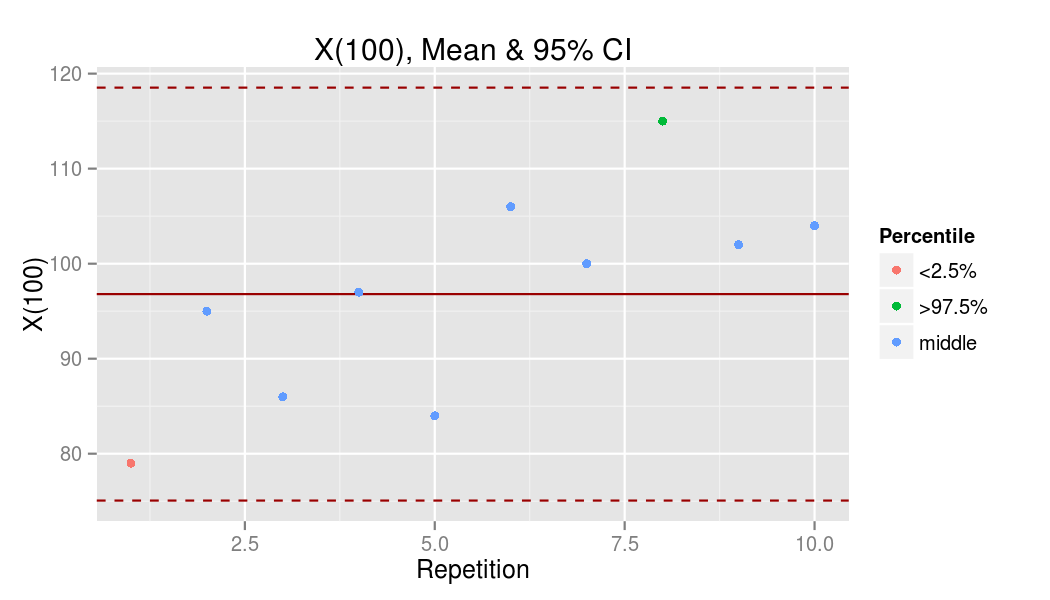
\includegraphics[width=.8\linewidth]{figure/many2} 

\end{knitrout}


Mean and CI for the last sample:
\begin{knitrout}
\definecolor{shadecolor}{rgb}{0.969, 0.969, 0.969}\color{fgcolor}\begin{kframe}
\begin{alltt}
\hlkwd{print}\hlstd{(}\hlkwd{paste}\hlstd{(}\hlstr{"Mean:"}\hlstd{,} \hlkwd{round}\hlstd{(mean_sd}\hlopt{$}\hlstd{mean),} \hlstr{"  95% CI["}\hlstd{,} \hlkwd{round}\hlstd{(mean_sd}\hlopt{$}\hlstd{mean} \hlopt{-}
    \hlstd{mean_sd}\hlopt{$}\hlstd{sd} \hlopt{*} \hlnum{1.9604}\hlstd{),} \hlstr{","}\hlstd{,} \hlkwd{round}\hlstd{(mean_sd}\hlopt{$}\hlstd{mean} \hlopt{+} \hlstd{mean_sd}\hlopt{$}\hlstd{sd} \hlopt{*} \hlnum{1.9604}\hlstd{),} \hlstr{"]"}\hlstd{))}
\end{alltt}
\begin{verbatim}
[1] "Mean: 97   95% CI[ 75 , 119 ]"
\end{verbatim}
\end{kframe}
\end{knitrout}

Percentiles for the last sample:
\begin{knitrout}
\definecolor{shadecolor}{rgb}{0.969, 0.969, 0.969}\color{fgcolor}\begin{kframe}
\begin{alltt}
\hlkwd{print}\hlstd{(median_quantiles)}
\end{alltt}
\begin{verbatim}
  2.5%    50%  97.5% 
 80.12  98.50 112.98 
\end{verbatim}
\end{kframe}
\end{knitrout}

Max of the last sample \& max of the highest value within repetitions:
\begin{knitrout}
\definecolor{shadecolor}{rgb}{0.969, 0.969, 0.969}\color{fgcolor}\begin{kframe}
\begin{alltt}
\hlkwd{print}\hlstd{(}\hlkwd{paste}\hlstd{(}\hlstr{"Max[X(100)]:"}\hlstd{,} \hlkwd{max}\hlstd{(within_summary}\hlopt{$}\hlstd{X_end)))}
\end{alltt}
\begin{verbatim}
[1] "Max[X(100)]: 115"
\end{verbatim}
\begin{alltt}
\hlkwd{print}\hlstd{(}\hlkwd{paste}\hlstd{(}\hlstr{"Max[Highest_X]:"}\hlstd{,} \hlkwd{max}\hlstd{(within_summary}\hlopt{$}\hlstd{X_max)))}
\end{alltt}
\begin{verbatim}
[1] "Max[Highest_X]: 150"
\end{verbatim}
\end{kframe}
\end{knitrout}


\bf{5 Comparing Logistic \& SI models}
\begin{knitrout}
\definecolor{shadecolor}{rgb}{0.969, 0.969, 0.969}\color{fgcolor}\begin{kframe}
\begin{alltt}
\hlkwd{rm}\hlstd{(}\hlkwc{list} \hlstd{=} \hlkwd{ls}\hlstd{(}\hlkwc{all} \hlstd{=} \hlnum{TRUE}\hlstd{))}
\hlstd{sim_out} \hlkwb{<-} \hlkwd{data.frame}\hlstd{(}\hlkwc{Repetition} \hlstd{=} \hlkwd{numeric}\hlstd{(),} \hlkwc{Sample} \hlstd{=} \hlkwd{numeric}\hlstd{(),} \hlkwc{Time} \hlstd{=} \hlkwd{numeric}\hlstd{(),}
    \hlkwc{X} \hlstd{=} \hlkwd{numeric}\hlstd{(),} \hlkwc{Model} \hlstd{=} \hlkwd{character}\hlstd{())}

\hlcom{## Defining constants}
\hlstd{parms} \hlkwb{<-} \hlkwd{c}\hlstd{(}\hlkwc{c1} \hlstd{=} \hlnum{1}\hlstd{,} \hlkwc{c2} \hlstd{=} \hlnum{0.1}\hlstd{,} \hlkwc{r} \hlstd{=} \hlnum{0.1}\hlstd{)}
\hlstd{init} \hlkwb{<-} \hlkwd{c}\hlstd{(}\hlkwc{X} \hlstd{=} \hlnum{1}\hlstd{,} \hlkwc{S} \hlstd{=} \hlnum{99}\hlstd{,} \hlkwc{I} \hlstd{=} \hlnum{1}\hlstd{)}

\hlcom{## Deterministic Logistic & SI model}
\hlstd{deriv} \hlkwb{<-} \hlkwa{function}\hlstd{(}\hlkwc{time}\hlstd{,} \hlkwc{state}\hlstd{,} \hlkwc{parameters}\hlstd{) \{}
    \hlkwd{with}\hlstd{(}\hlkwd{as.list}\hlstd{(}\hlkwd{c}\hlstd{(state, parameters)), \{}
        \hlstd{dX} \hlkwb{<-} \hlstd{c1} \hlopt{*} \hlstd{X} \hlopt{-} \hlstd{c2} \hlopt{*} \hlstd{X} \hlopt{*} \hlstd{X}
        \hlstd{dS} \hlkwb{<-} \hlopt{-}\hlstd{r} \hlopt{*} \hlstd{I} \hlopt{*} \hlstd{S}
        \hlstd{dI} \hlkwb{<-} \hlstd{r} \hlopt{*} \hlstd{I} \hlopt{*} \hlstd{S}
        \hlkwd{return}\hlstd{(}\hlkwd{list}\hlstd{(}\hlkwd{c}\hlstd{(dX, dS, dI)))}
    \hlstd{\})}
\hlstd{\}}
\hlstd{times} \hlkwb{<-} \hlkwd{seq}\hlstd{(}\hlnum{0}\hlstd{,} \hlnum{20}\hlstd{,} \hlkwc{by} \hlstd{=} \hlnum{0.01}\hlstd{)}
\hlstd{out} \hlkwb{<-} \hlkwd{as.data.frame}\hlstd{(}\hlkwd{ode}\hlstd{(}\hlkwc{y} \hlstd{= init,} \hlkwc{times} \hlstd{= times,} \hlkwc{func} \hlstd{= deriv,} \hlkwc{parms} \hlstd{= parms))}
\hlstd{Repetition} \hlkwb{<-} \hlkwd{rep}\hlstd{(}\hlnum{1}\hlstd{,} \hlkwd{nrow}\hlstd{(out))}
\hlstd{Sample} \hlkwb{<-} \hlnum{1}\hlopt{:}\hlkwd{nrow}\hlstd{(out)}
\hlstd{sim_out} \hlkwb{<-} \hlkwd{rbind}\hlstd{(sim_out,} \hlkwd{data.frame}\hlstd{(Repetition, Sample,} \hlkwc{Time} \hlstd{= times,} \hlkwc{X} \hlstd{= out}\hlopt{$}\hlstd{X,}
    \hlkwc{Model} \hlstd{=} \hlkwd{rep}\hlstd{(}\hlstr{"Deterministic Logistic Model"}\hlstd{,} \hlkwd{nrow}\hlstd{(out))))}
\hlstd{sim_out} \hlkwb{<-} \hlkwd{rbind}\hlstd{(sim_out,} \hlkwd{data.frame}\hlstd{(Repetition, Sample,} \hlkwc{Time} \hlstd{= times,} \hlkwc{X} \hlstd{= out}\hlopt{$}\hlstd{I,}
    \hlkwc{Model} \hlstd{=} \hlkwd{rep}\hlstd{(}\hlstr{"Deterministic SI Model"}\hlstd{,} \hlkwd{nrow}\hlstd{(out))))}

\hlcom{## Stochastic Logistic & SI model}
\hlkwa{for} \hlstd{(i} \hlkwa{in} \hlnum{1}\hlopt{:}\hlnum{10}\hlstd{) \{}
    \hlstd{a} \hlkwb{<-} \hlkwd{c}\hlstd{(}\hlstr{"c1 * X"}\hlstd{,} \hlstr{"c2 * X * X"}\hlstd{,} \hlstr{"r*S*I"}\hlstd{)}
    \hlstd{nu} \hlkwb{<-} \hlkwd{matrix}\hlstd{(}\hlkwd{c}\hlstd{(}\hlopt{+}\hlnum{1}\hlstd{,} \hlopt{-}\hlnum{1}\hlstd{,} \hlnum{0}\hlstd{,} \hlnum{0}\hlstd{,} \hlnum{0}\hlstd{,} \hlopt{-}\hlnum{1}\hlstd{,} \hlnum{0}\hlstd{,} \hlnum{0}\hlstd{,} \hlopt{+}\hlnum{1}\hlstd{),} \hlkwc{nrow} \hlstd{=} \hlnum{3}\hlstd{,} \hlkwc{byrow} \hlstd{= T)}
    \hlstd{out} \hlkwb{<-} \hlkwd{ssa}\hlstd{(init, a, nu, parms,} \hlkwc{tf} \hlstd{=} \hlnum{20}\hlstd{,} \hlkwc{tau} \hlstd{=} \hlnum{0.01}\hlstd{,} \hlkwc{method} \hlstd{=} \hlstr{"ETL"}\hlstd{,} \hlkwc{maxWallTime} \hlstd{=} \hlnum{5}\hlstd{,}
        \hlkwc{ignoreNegativeState} \hlstd{= T)}
    \hlcom{#'Explicit tau-leap' => user-defined step size}
    \hlcom{# ignoreNegativeState => gives warning instead of error for negative number}
    \hlcom{# of susceptibles.}
    \hlstd{Repetition} \hlkwb{<-} \hlkwd{rep}\hlstd{(i,} \hlkwd{nrow}\hlstd{(out}\hlopt{$}\hlstd{data))}
    \hlstd{Sample} \hlkwb{<-} \hlnum{1}\hlopt{:}\hlkwd{nrow}\hlstd{(out}\hlopt{$}\hlstd{data)}
    \hlstd{sim_out} \hlkwb{<-} \hlkwd{rbind}\hlstd{(sim_out,} \hlkwd{data.frame}\hlstd{(Repetition, Sample,} \hlkwc{Time} \hlstd{= out}\hlopt{$}\hlstd{data[,}
        \hlnum{1}\hlstd{],} \hlkwc{X} \hlstd{= out}\hlopt{$}\hlstd{data[,} \hlnum{2}\hlstd{],} \hlkwc{Model} \hlstd{=} \hlkwd{rep}\hlstd{(}\hlstr{"Stochastic Logistic Model"}\hlstd{,} \hlkwd{nrow}\hlstd{(out}\hlopt{$}\hlstd{data))))}
    \hlstd{sim_out} \hlkwb{<-} \hlkwd{rbind}\hlstd{(sim_out,} \hlkwd{data.frame}\hlstd{(Repetition, Sample,} \hlkwc{Time} \hlstd{= out}\hlopt{$}\hlstd{data[,}
        \hlnum{1}\hlstd{],} \hlkwc{X} \hlstd{= out}\hlopt{$}\hlstd{data[,} \hlnum{4}\hlstd{],} \hlkwc{Model} \hlstd{=} \hlkwd{rep}\hlstd{(}\hlstr{"Stochastic SI Model"}\hlstd{,} \hlkwd{nrow}\hlstd{(out}\hlopt{$}\hlstd{data))))}
\hlstd{\}}
\hlstd{within_summary} \hlkwb{<-} \hlkwd{ddply}\hlstd{(sim_out,} \hlkwd{.}\hlstd{(Model, Repetition), summarise,} \hlkwc{X_end} \hlstd{=} \hlkwd{tail}\hlstd{(X,}
    \hlkwc{n} \hlstd{=} \hlnum{1}\hlstd{))}

\hlcom{## Plot results}
\hlkwd{ggplot}\hlstd{(sim_out,} \hlkwd{aes}\hlstd{(}\hlkwc{x} \hlstd{= Time,} \hlkwc{y} \hlstd{= X,} \hlkwc{colour} \hlstd{= Repetition))} \hlopt{+} \hlkwd{geom_line}\hlstd{(}\hlkwd{aes}\hlstd{(}\hlkwc{group} \hlstd{= Repetition))} \hlopt{+}
    \hlkwd{facet_wrap}\hlstd{(}\hlopt{~}\hlstd{Model,} \hlkwc{ncol} \hlstd{=} \hlnum{2}\hlstd{)}
\end{alltt}
\end{kframe}
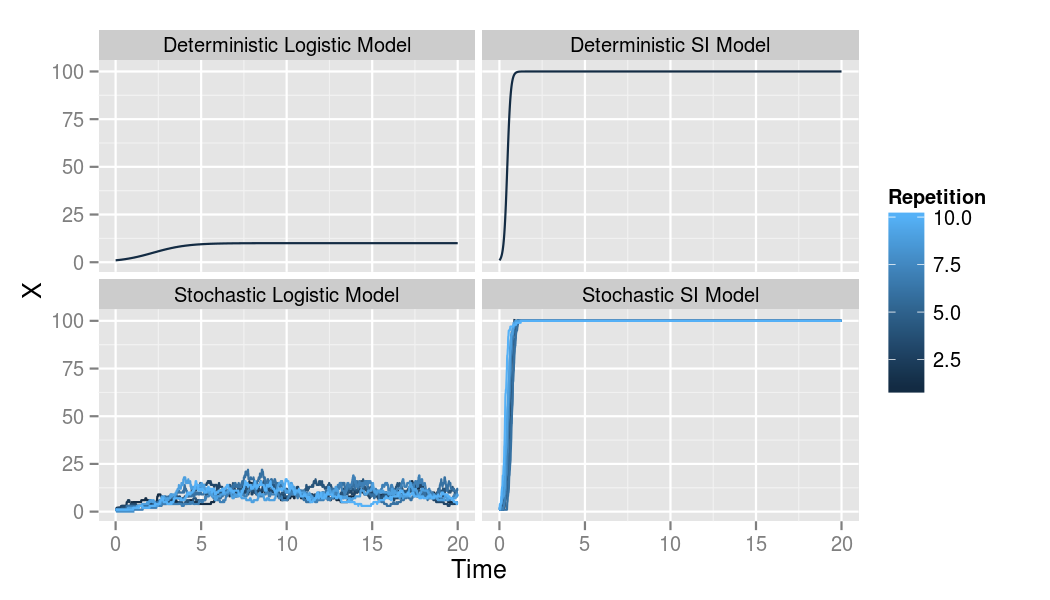
\includegraphics[width=.8\linewidth]{figure/Log_SI1} 
\begin{kframe}\begin{alltt}
\hlstd{mean_sd} \hlkwb{<-} \hlkwd{ddply}\hlstd{(within_summary,} \hlkwd{.}\hlstd{(Model), summarise,} \hlkwc{mean} \hlstd{=} \hlkwd{mean}\hlstd{(X_end,} \hlkwc{na.rm} \hlstd{=} \hlnum{TRUE}\hlstd{),}
    \hlkwc{sd} \hlstd{=} \hlkwd{sd}\hlstd{(X_end,} \hlkwc{na.rm} \hlstd{=} \hlnum{TRUE}\hlstd{))}
\hlstd{plot_end} \hlkwb{<-} \hlkwd{ggplot}\hlstd{(}\hlkwc{data} \hlstd{= within_summary,} \hlkwd{aes}\hlstd{(}\hlkwc{x} \hlstd{= Repetition,} \hlkwc{y} \hlstd{= X_end))} \hlopt{+}
    \hlkwd{geom_point}\hlstd{()}
\hlstd{plot_end} \hlopt{+} \hlkwd{geom_hline}\hlstd{(}\hlkwc{data} \hlstd{= mean_sd,} \hlkwd{aes}\hlstd{(}\hlkwc{yintercept} \hlstd{= mean,} \hlnum{3}\hlstd{),} \hlkwc{linetype} \hlstd{=} \hlnum{1}\hlstd{,}
    \hlkwc{colour} \hlstd{=} \hlstr{"#990000"}\hlstd{)}
\end{alltt}
\end{kframe}
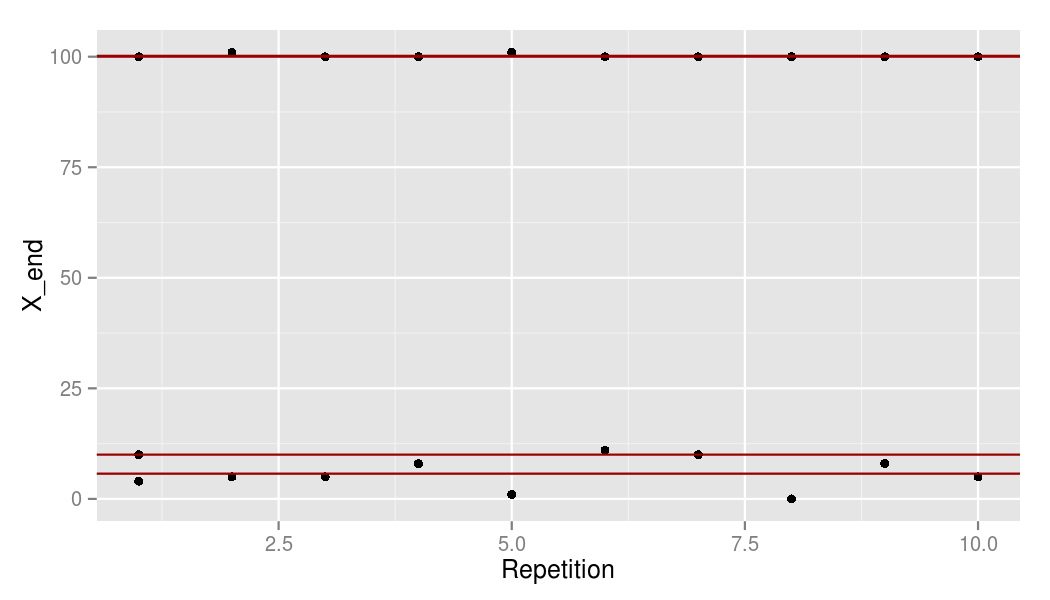
\includegraphics[width=.8\linewidth]{figure/Log_SI2} 
\begin{kframe}\begin{alltt}
\hlstd{plot_end} \hlopt{+} \hlkwd{geom_hline}\hlstd{(}\hlkwc{data} \hlstd{= mean_sd,} \hlkwd{aes}\hlstd{(}\hlkwc{yintercept} \hlstd{= mean} \hlopt{+} \hlnum{1.9604} \hlopt{*} \hlstd{sd,} \hlnum{3}\hlstd{),}
    \hlkwc{linetype} \hlstd{=} \hlnum{2}\hlstd{,} \hlkwc{colour} \hlstd{=} \hlstr{"#990000"}\hlstd{)}
\end{alltt}
\end{kframe}
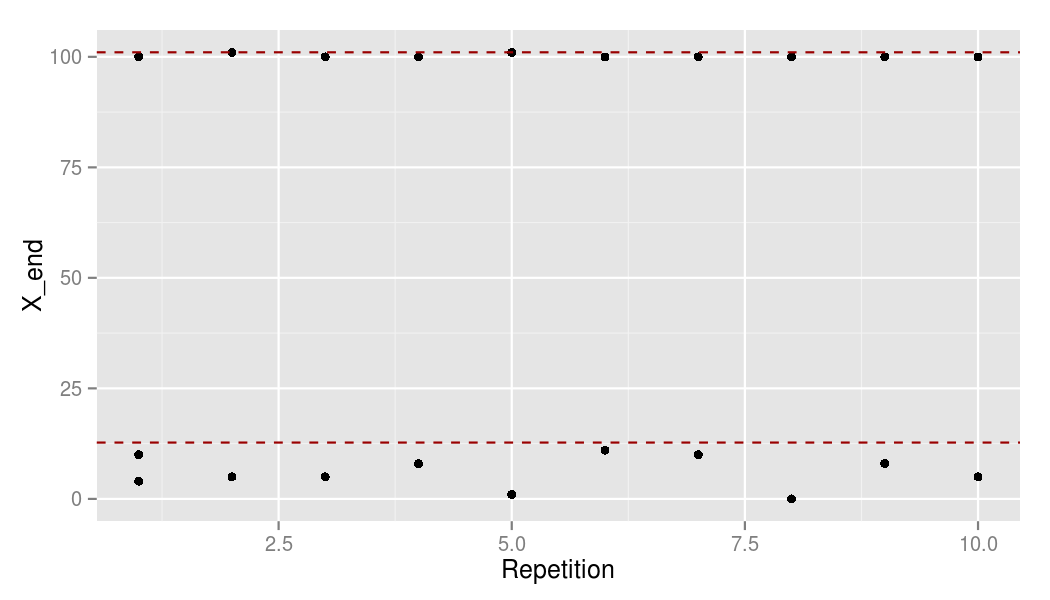
\includegraphics[width=.8\linewidth]{figure/Log_SI3} 
\begin{kframe}\begin{alltt}
\hlstd{plot_end} \hlopt{+} \hlkwd{geom_hline}\hlstd{(}\hlkwc{data} \hlstd{= mean_sd,} \hlkwd{aes}\hlstd{(}\hlkwc{yintercept} \hlstd{= mean} \hlopt{-} \hlnum{1.9604} \hlopt{*} \hlstd{sd,} \hlnum{3}\hlstd{),}
    \hlkwc{linetype} \hlstd{=} \hlnum{2}\hlstd{,} \hlkwc{colour} \hlstd{=} \hlstr{"#990000"}\hlstd{)}
\end{alltt}
\end{kframe}
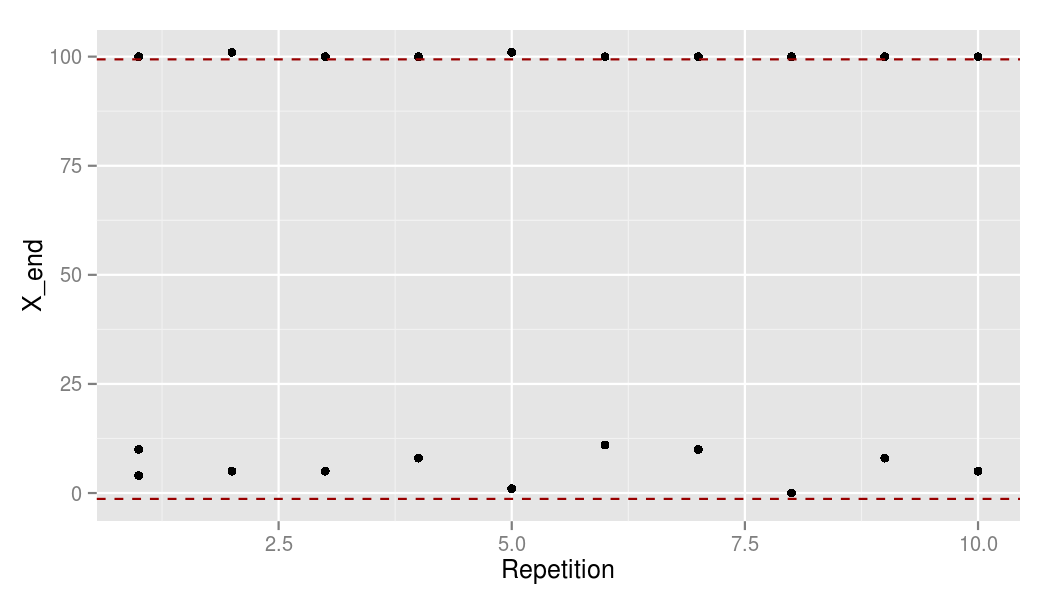
\includegraphics[width=.8\linewidth]{figure/Log_SI4} 
\begin{kframe}\begin{alltt}
\hlstd{plot_end} \hlopt{+} \hlkwd{facet_wrap}\hlstd{(}\hlopt{~}\hlstd{Model,} \hlkwc{ncol} \hlstd{=} \hlnum{2}\hlstd{)} \hlopt{+} \hlkwd{ggtitle}\hlstd{(}\hlstr{"X(20), Mean & 95% CI"}\hlstd{)} \hlopt{+}
    \hlkwd{ylab}\hlstd{(}\hlstr{"X(20)"}\hlstd{)}
\end{alltt}
\end{kframe}
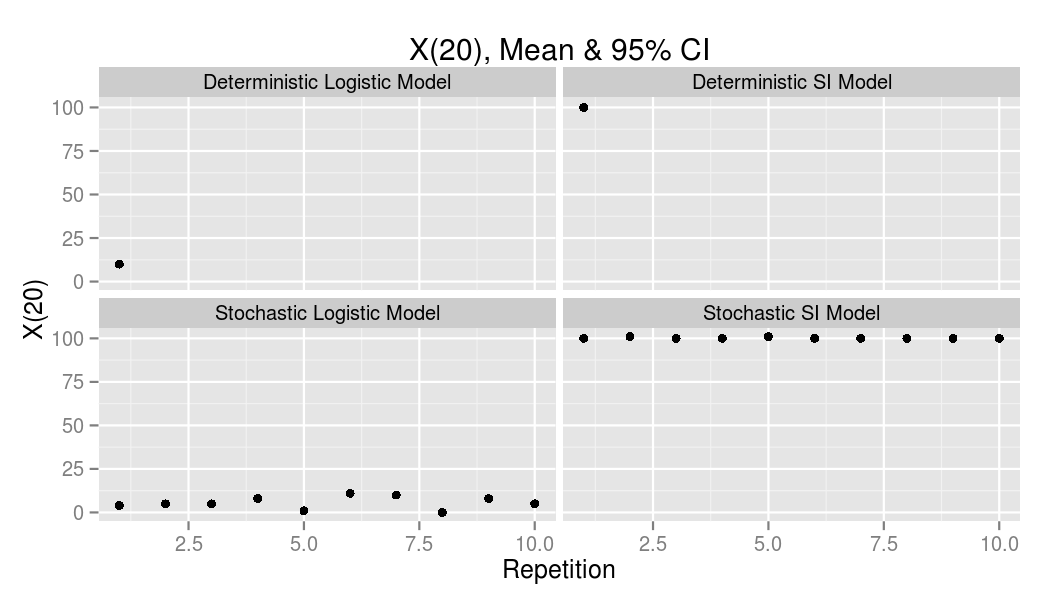
\includegraphics[width=.8\linewidth]{figure/Log_SI5} 

\end{knitrout}


Summarising the effects of changing dt:
\begin{knitrout}
\definecolor{shadecolor}{rgb}{0.969, 0.969, 0.969}\color{fgcolor}\begin{kframe}
\begin{alltt}
\hlcom{# End sample summary}
\hlstd{End_summary} \hlkwb{<-} \hlkwd{ddply}\hlstd{(within_summary,} \hlkwd{.}\hlstd{(Model), summarise,} \hlkwc{Av_end_X} \hlstd{=} \hlkwd{mean}\hlstd{(X_end),}
    \hlkwc{CI_low} \hlstd{=} \hlkwd{mean}\hlstd{(X_end)} \hlopt{-} \hlnum{1.9604} \hlopt{*} \hlkwd{sd}\hlstd{(X_end),} \hlkwc{CI_high} \hlstd{=} \hlkwd{mean}\hlstd{(X_end)} \hlopt{+} \hlnum{1.9604} \hlopt{*}
        \hlkwd{sd}\hlstd{(X_end))}
\hlkwd{print}\hlstd{(}\hlstr{"Last sample summary:"}\hlstd{)}
\end{alltt}
\begin{verbatim}
[1] "Last sample summary:"
\end{verbatim}
\begin{alltt}
\hlkwd{print}\hlstd{(End_summary)}
\end{alltt}
\begin{verbatim}
                         Model Av_end_X CI_low CI_high
1 Deterministic Logistic Model     10.0     NA      NA
2       Deterministic SI Model    100.0     NA      NA
3    Stochastic Logistic Model      5.7 -1.341   12.74
4          Stochastic SI Model    100.2 99.373  101.03
\end{verbatim}
\begin{alltt}
\hlcom{# Percent Extinction summary}
\hlstd{PercentExtinct} \hlkwb{<-} \hlkwd{ddply}\hlstd{(within_summary,} \hlkwd{.}\hlstd{(Model), summarise,} \hlkwc{PercentExtinct} \hlstd{=} \hlkwd{length}\hlstd{(X_end[X_end} \hlopt{<}
    \hlnum{0.5}\hlstd{])}\hlopt{/}\hlkwd{length}\hlstd{(X_end)} \hlopt{*} \hlnum{100}\hlstd{)}
\hlkwd{print}\hlstd{(PercentExtinct)}
\end{alltt}
\begin{verbatim}
                         Model PercentExtinct
1 Deterministic Logistic Model              0
2       Deterministic SI Model              0
3    Stochastic Logistic Model             10
4          Stochastic SI Model              0
\end{verbatim}
\begin{alltt}
\hlcom{# End sample summary (discriminating extinct)}
\hlstd{No_ext_End_summary} \hlkwb{<-} \hlkwd{ddply}\hlstd{(within_summary[within_summary}\hlopt{$}\hlstd{X_end} \hlopt{>} \hlnum{0.5}\hlstd{, ],} \hlkwd{.}\hlstd{(Model),}
    \hlstd{summarise,} \hlkwc{Av_end_X} \hlstd{=} \hlkwd{mean}\hlstd{(X_end),} \hlkwc{CI_low} \hlstd{=} \hlkwd{mean}\hlstd{(X_end)} \hlopt{-} \hlnum{1.9604} \hlopt{*} \hlkwd{sd}\hlstd{(X_end),}
    \hlkwc{CI_high} \hlstd{=} \hlkwd{mean}\hlstd{(X_end)} \hlopt{+} \hlnum{1.9604} \hlopt{*} \hlkwd{sd}\hlstd{(X_end))}
\hlkwd{print}\hlstd{(}\hlstr{"Last sample summary, without extinction:"}\hlstd{)}
\end{alltt}
\begin{verbatim}
[1] "Last sample summary, without extinction:"
\end{verbatim}
\begin{alltt}
\hlkwd{print}\hlstd{(No_ext_End_summary)}
\end{alltt}
\begin{verbatim}
                         Model Av_end_X CI_low CI_high
1 Deterministic Logistic Model   10.000     NA      NA
2       Deterministic SI Model  100.000     NA      NA
3    Stochastic Logistic Model    6.333  0.134   12.53
4          Stochastic SI Model  100.200 99.373  101.03
\end{verbatim}
\end{kframe}
\end{knitrout}


\end{document}
